\documentclass[english,11pt,a4paper]{article}
\usepackage[T1]{fontenc}
\usepackage{graphicx}
\usepackage{mathtools}
\usepackage{amssymb}
\usepackage{amsthm}
\usepackage{thmtools}
\usepackage{xcolor}
\usepackage{nameref}
\usepackage{babel}
\usepackage{authblk}
\usepackage{fourier}
\usepackage{indentfirst}
\usepackage{float}
\usepackage{subcaption}
\usepackage[colorlinks, urlcolor=blue]{hyperref}

\title{Introdução à Neurociência Computacional\\Lista de Exercícios 3}
\author{Paulo R. Sturion}
\begin{document}
	\maketitle
	
	\noindent Todos os códigos escritos para produzir os resultados dos exercícios a seguir estão disponibilizados de forma clara e organizada no repositório Github:
	
	\begin{center}
		\noindent \href{https://github.com/prsturion/intro-computational-neurosciene.git}{https://github.com/prsturion/intro-computational-neuroscience.git} \newline
	\end{center}
	
	\noindent\textbf{Questão 1. Corrente A.}\\
	
	\noindent \textbf{(a)} Faça gráficos dos estados estacionários $(X_{\infty}(V))$ e das constantes de tempo $(\tau_{X}(V))$ \textit{versus} $V$ para as variáveis de \textit{gating} do modelo de Connor e Stevens $(X = \{n, m, h, a, b\})$.
	
	\begin{figure}[H]
		\centering
		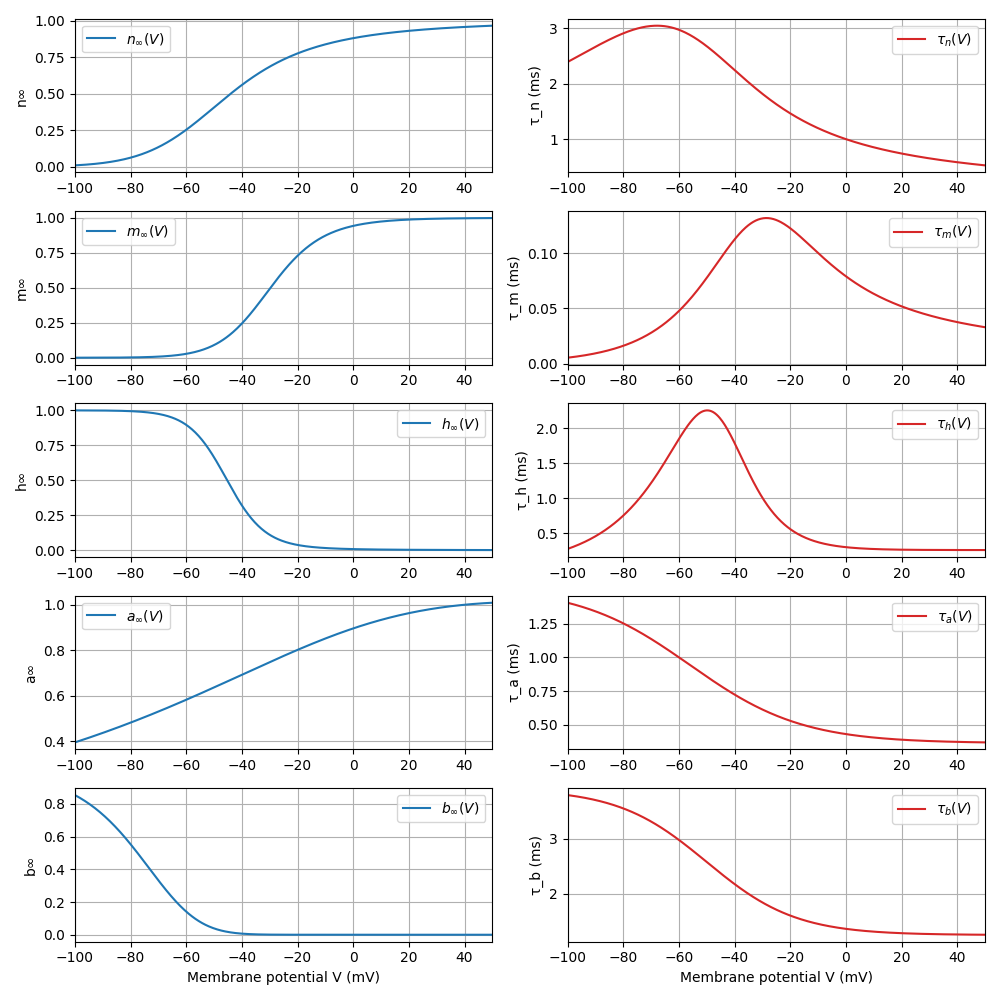
\includegraphics[width=13cm]{../figures/ex_1a.png}
		\caption{Graficos dos estados estacionários e das constantes de tempo das variáveis de \textit{gating} em função de $V$.}
	\end{figure}
	
	
	\noindent \textbf{(b)} Use as condições iniciais dadas por Ermentrout: $V(0) = -67{,}976 \ \text{mV}; \ n(0) = 0{,}1558; \ m(0) = 0{,}01; \ h(0) = 0{,}965; \ a(0) = 0{,}5404; \ e \ b(0) = 0{,}2885$. Resolva o sistema de EDOs do modelo de Connor e Stevens usando o método de Runge-Kutta de quarta ordem com passo de tempo de $0{,}01 \ \text{ms}$. Simule as equações do modelo de Connor-Stevens por um período de $200 \ \text{ms}$ começando das condições iniciais dadas acima e em $t = 60 \ \text{ms}$ injete uma densidade de corrente $J$ pelos restantes $140 \ \text{ms}$. Faça isso para quatro valores diferentes de $J$: $5, \ 10, \ 15 \ e \ 20 \ \mu A/\text{cm}^2$. Faça gráficos de $V, \ n, \ m, \ h, \ a \ e \ b$ em função de $t$ para essas quatro densidades de corrente injetada.\\
	
	\begin{figure}[H]
	\centering
	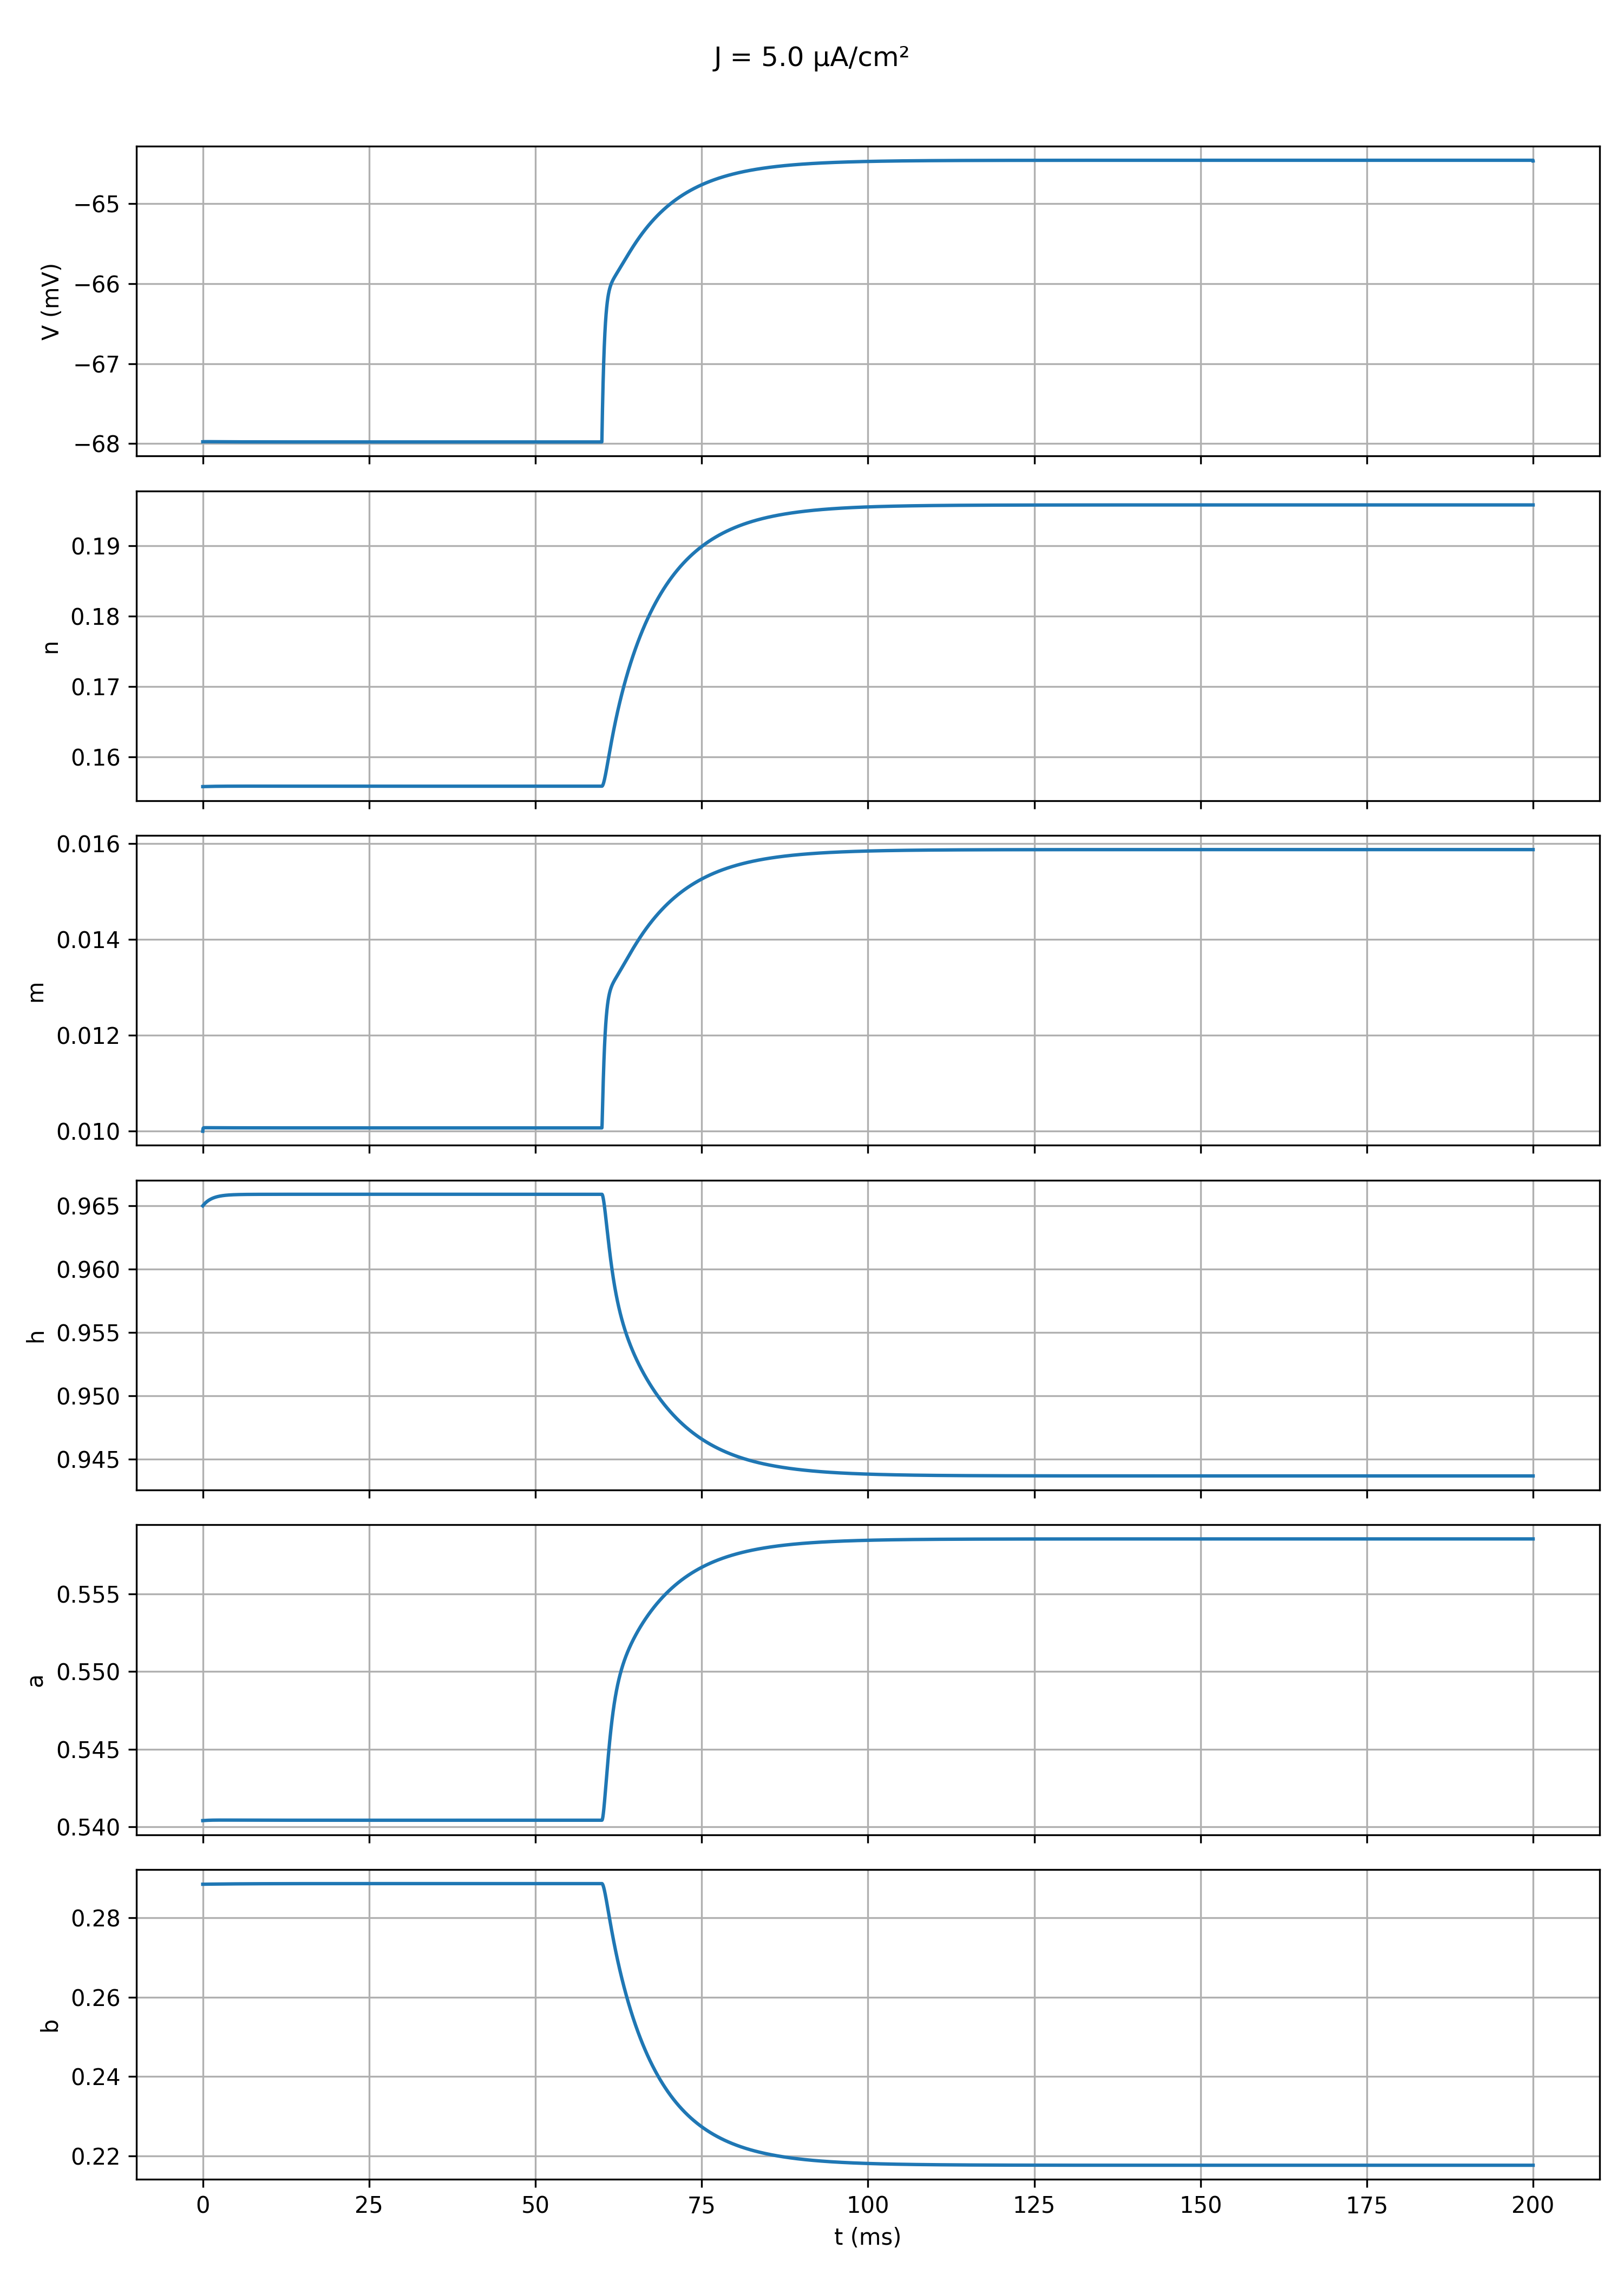
\includegraphics[width=11cm]{../figures/ex_1b_1.png}	
	\end{figure}

	\begin{figure}[H]
	\centering
	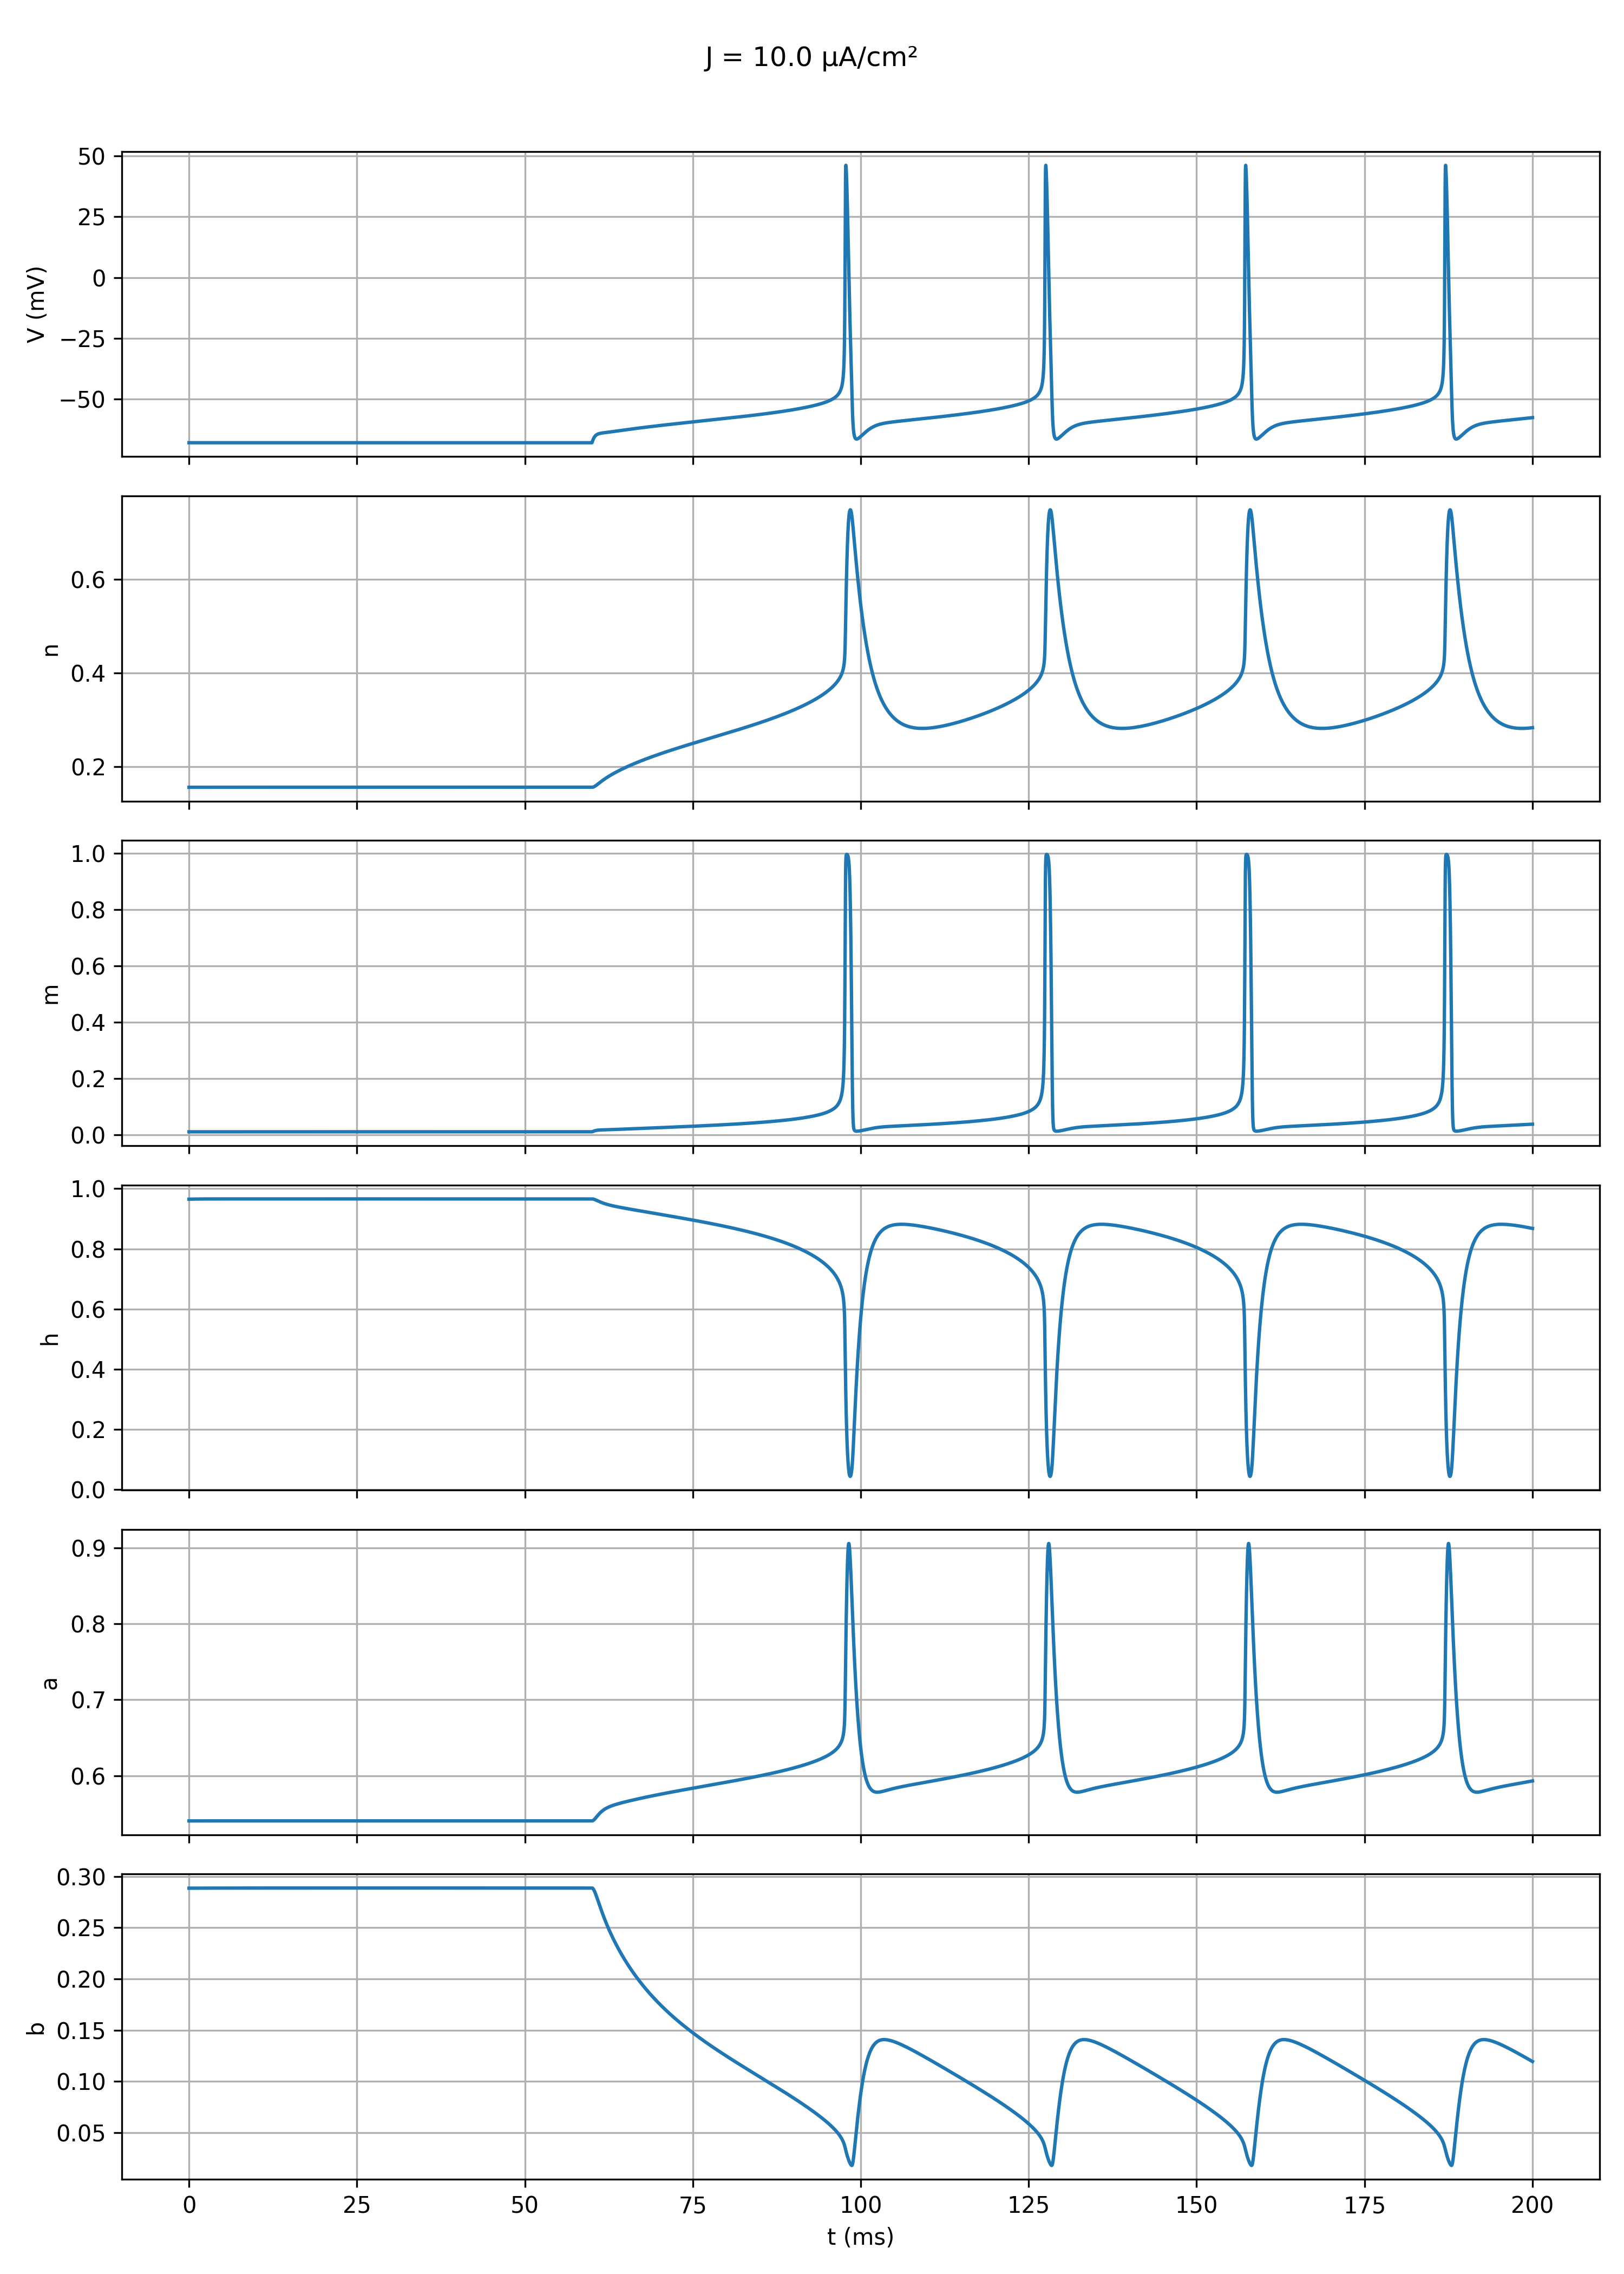
\includegraphics[width=11cm]{../figures/ex_1b_2.png}	
	\end{figure}

	\begin{figure}[H]
	\centering
	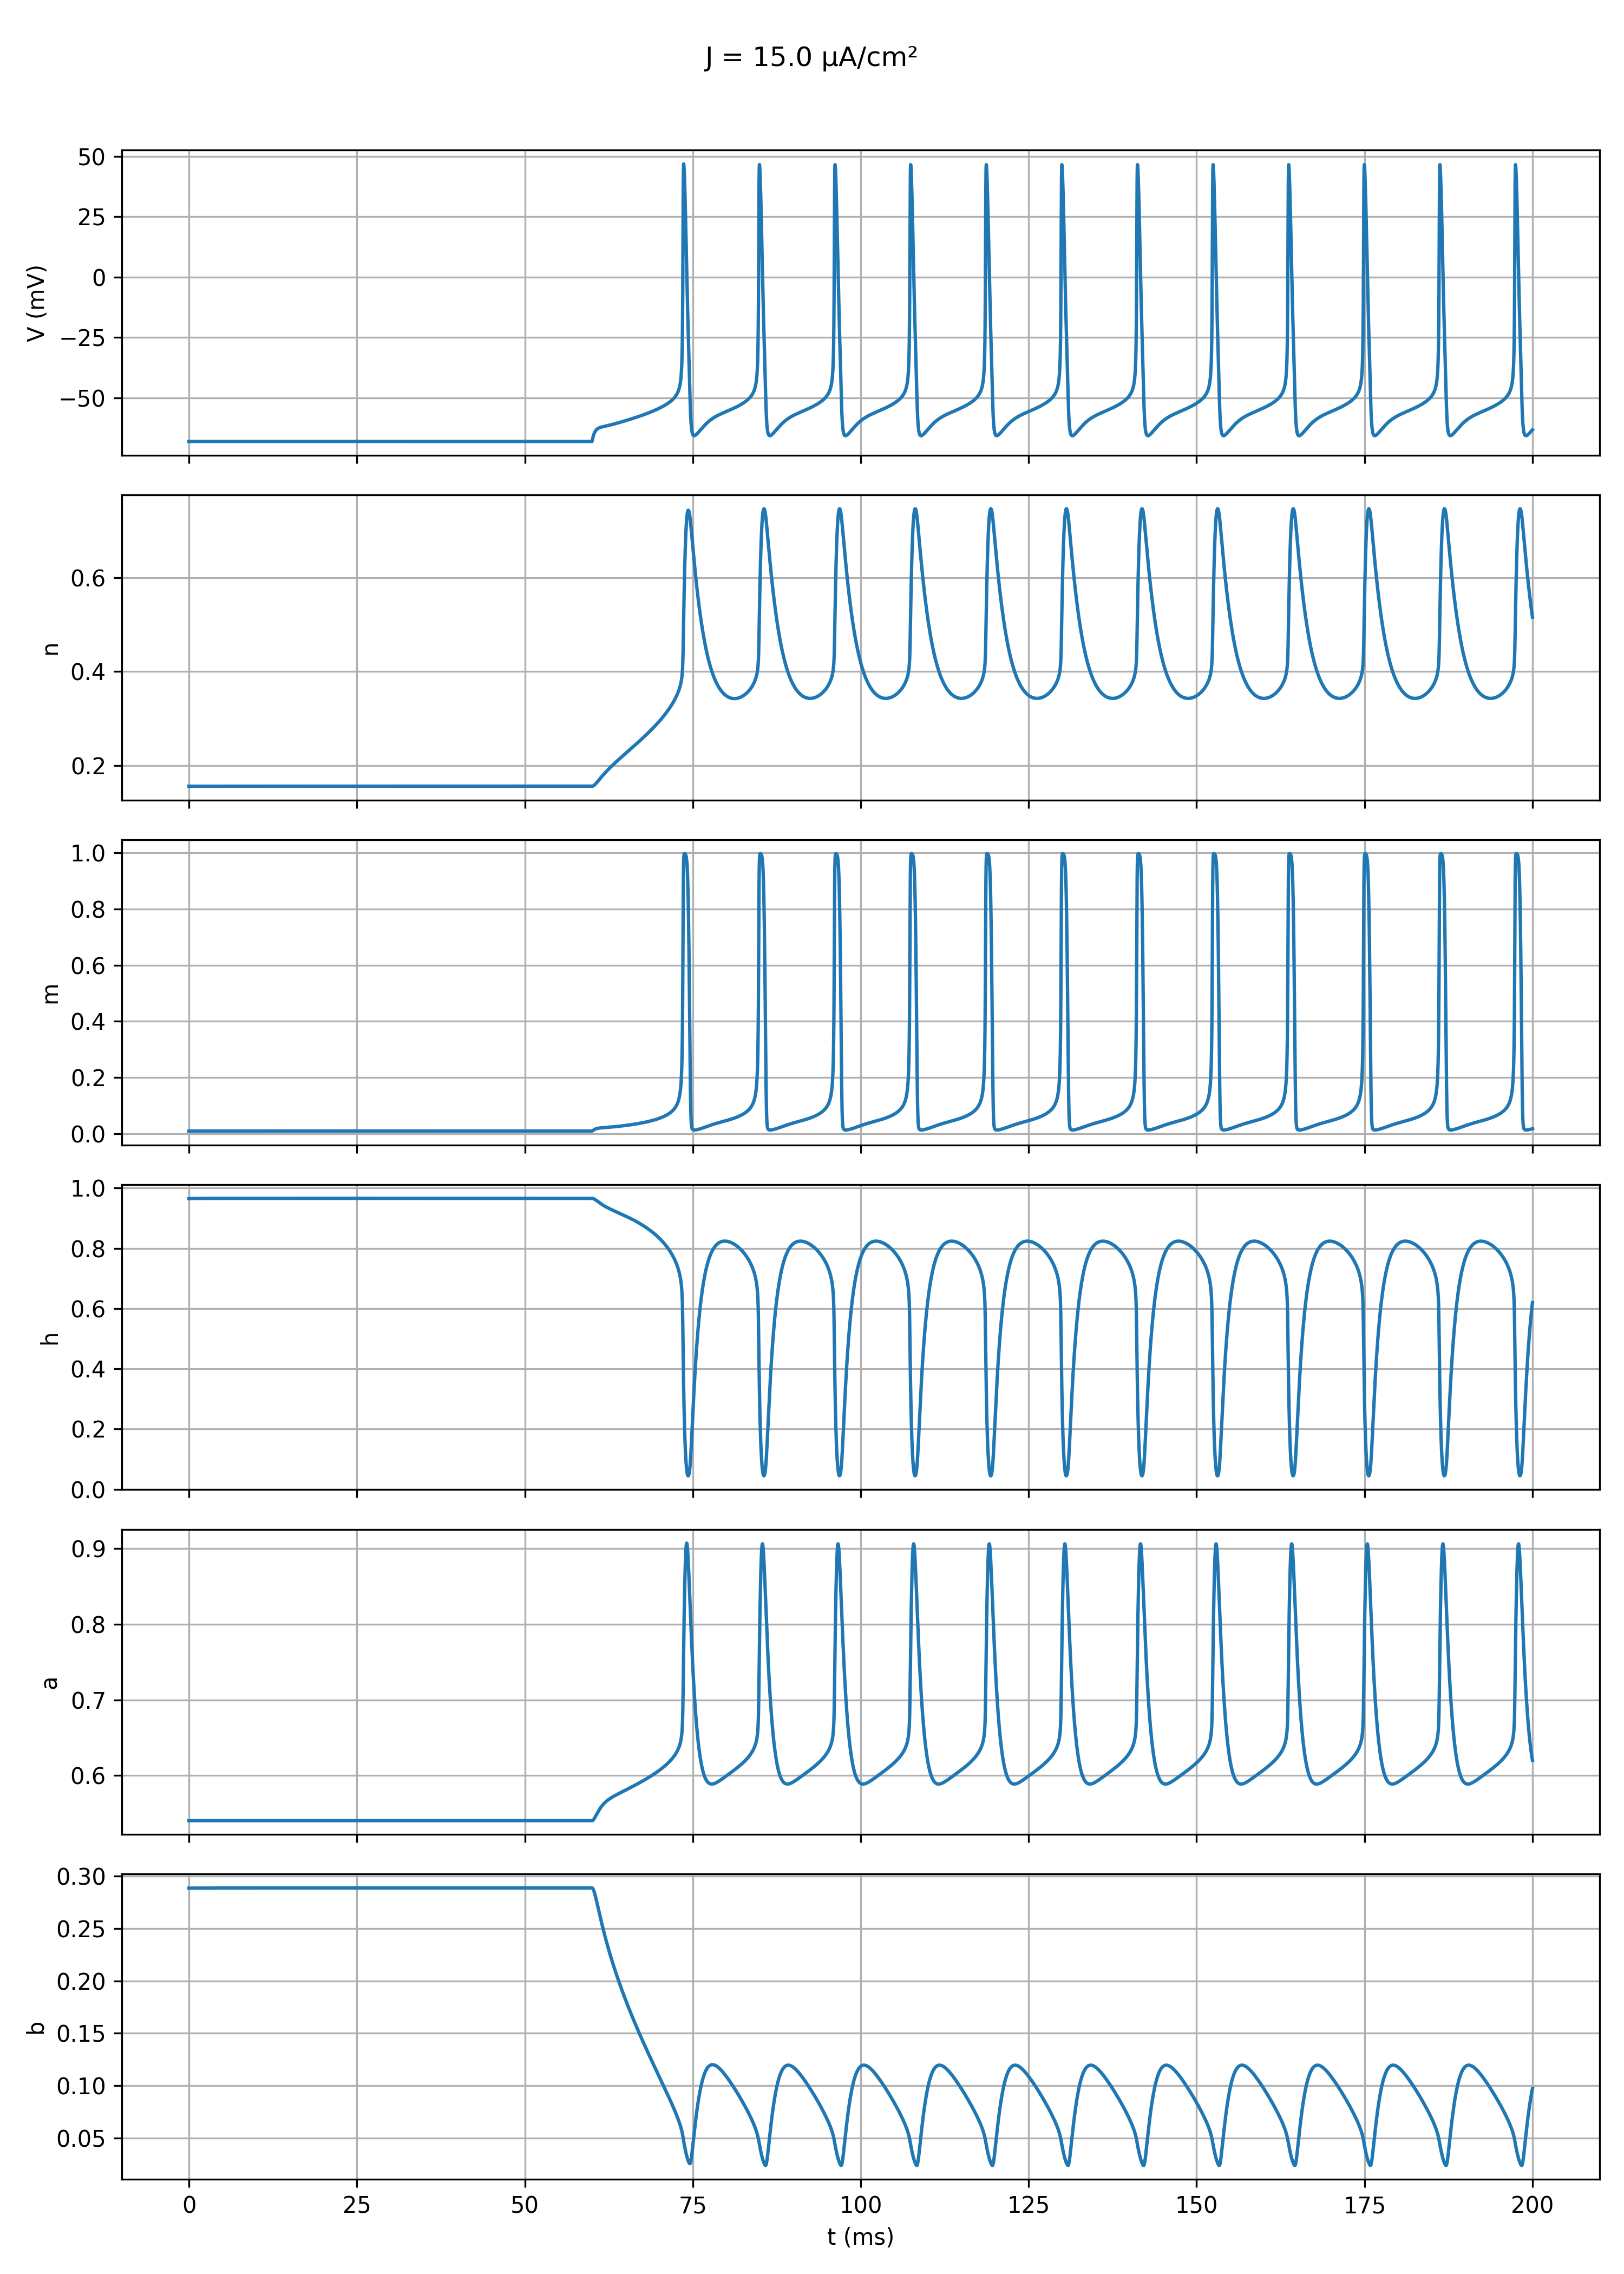
\includegraphics[width=11cm]{../figures/ex_1b_3.png}	
	\end{figure}

	\begin{figure}[H]
	\centering
	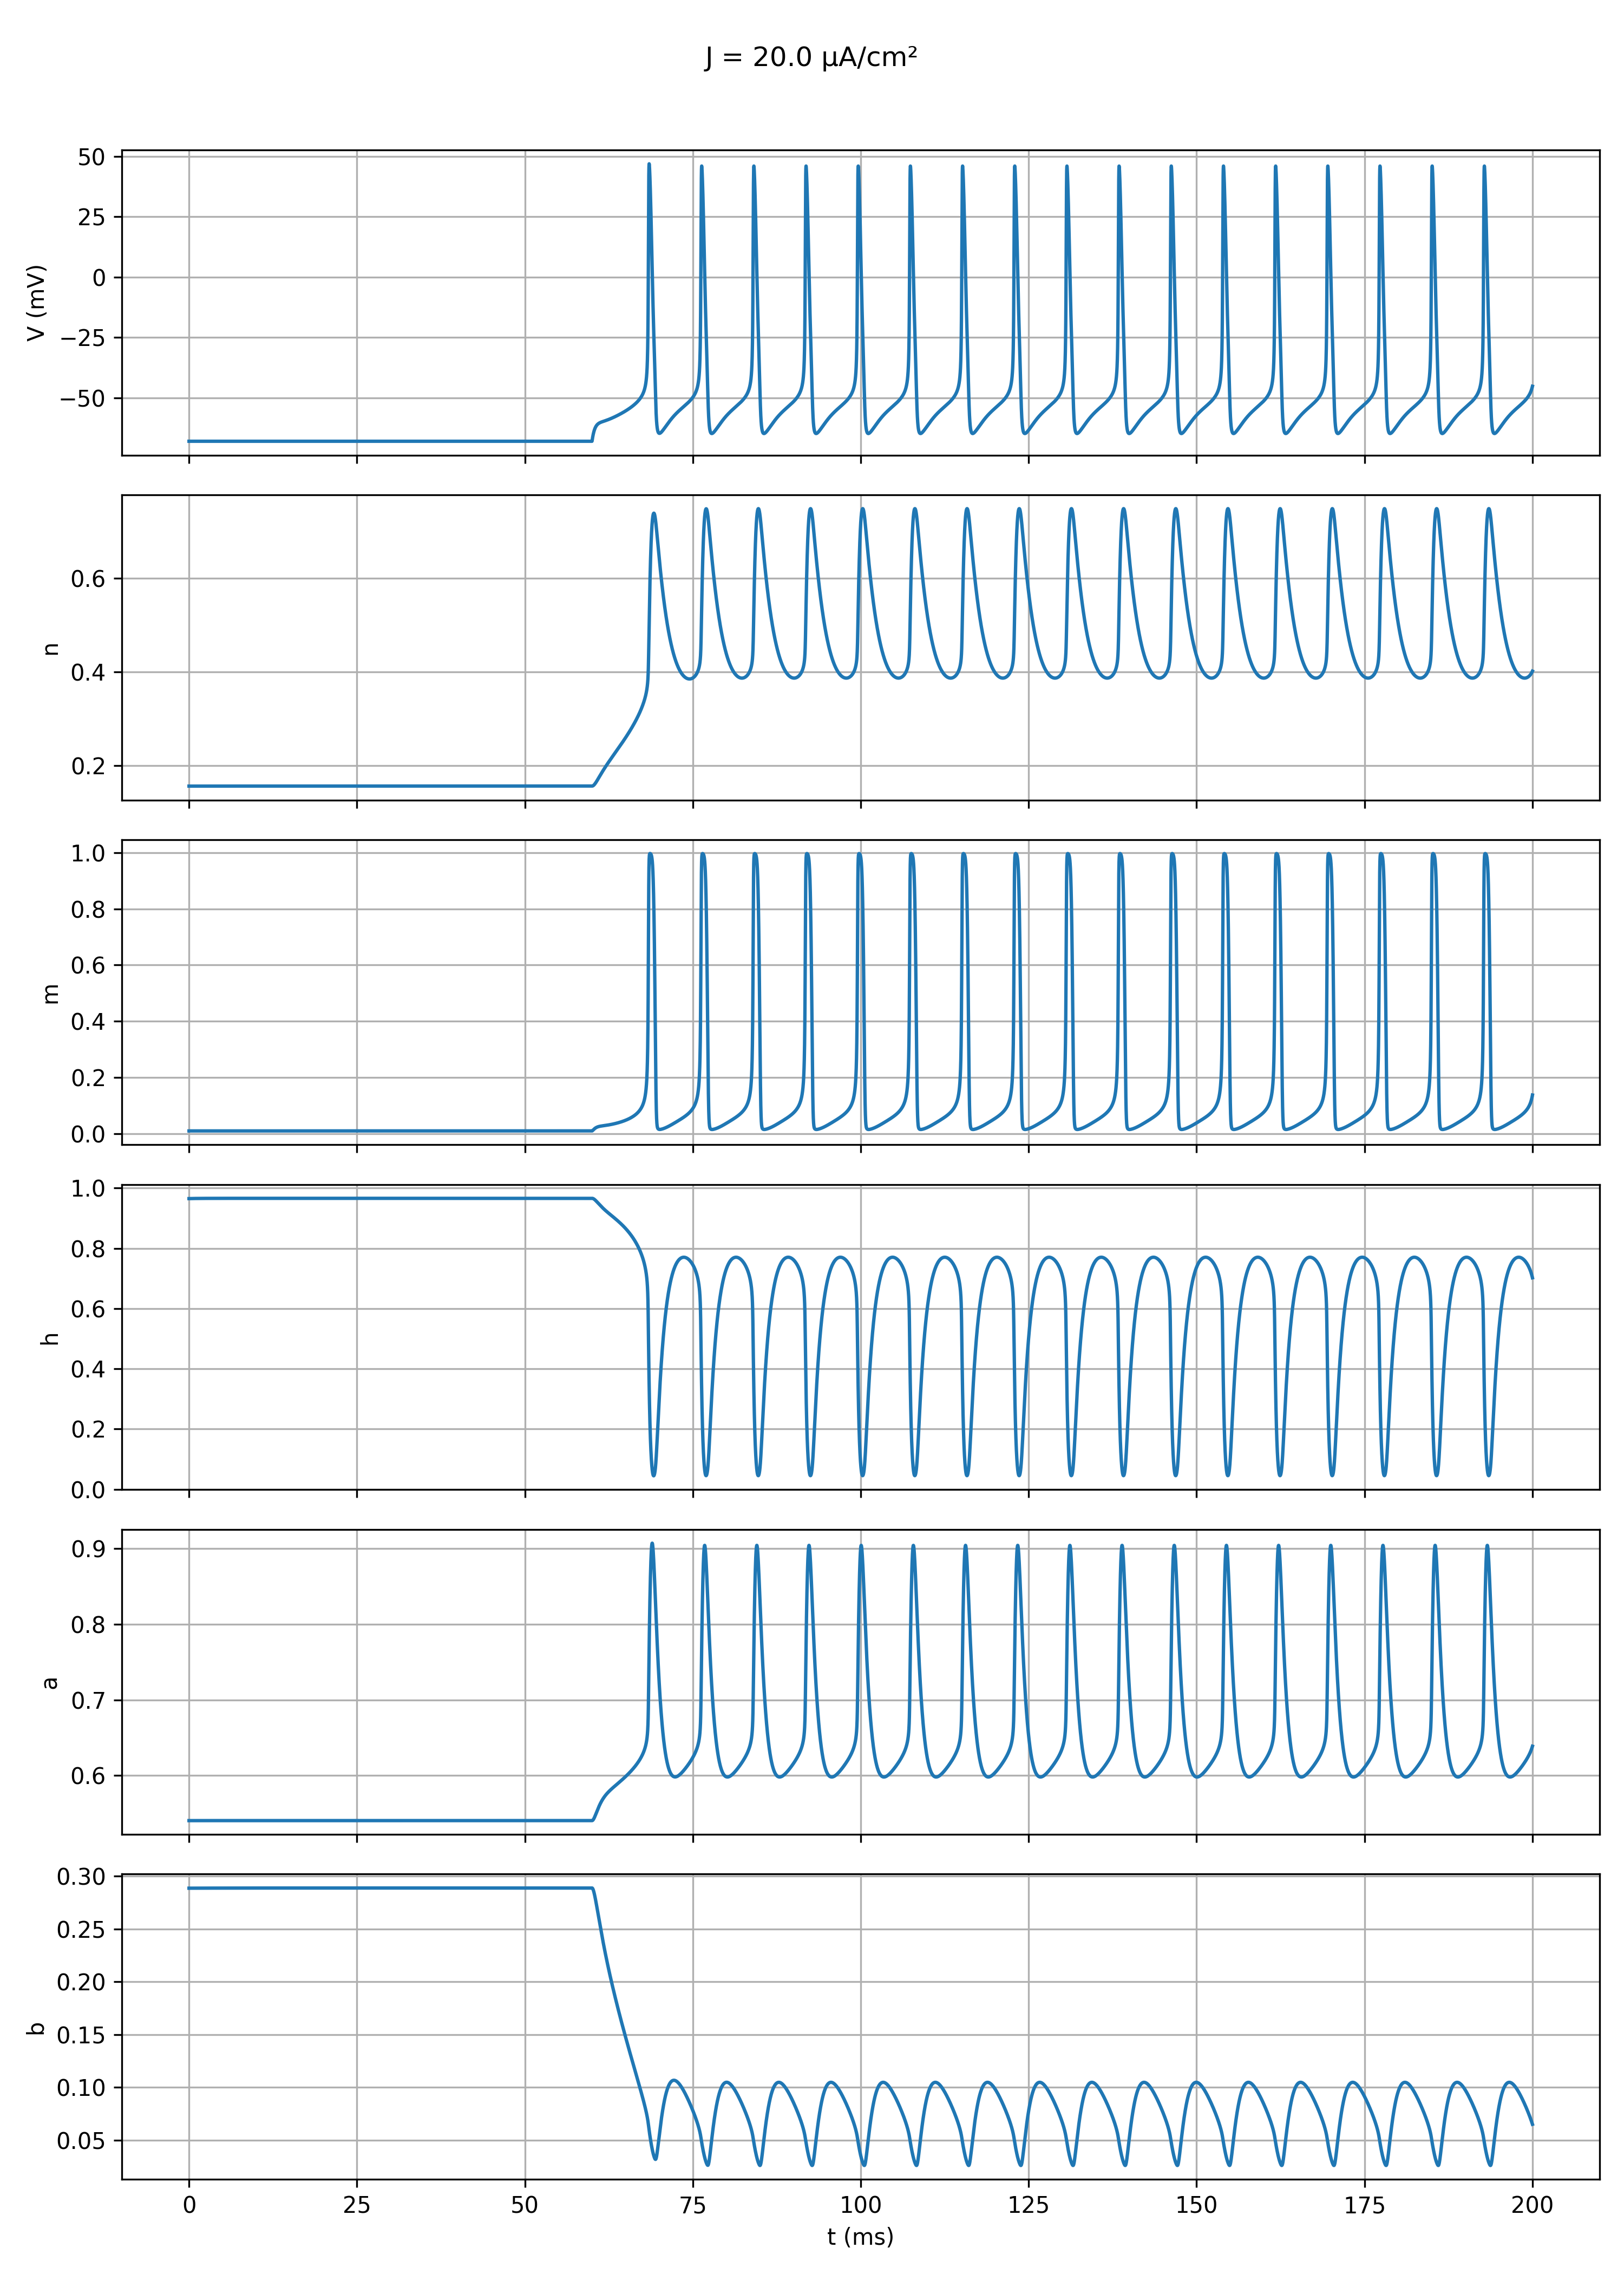
\includegraphics[width=11cm]{../figures/ex_1b_4.png}	
	\caption{Sequência de gráficos para $V$ e as variáveis de gating sujeitos a diferentes intensidades de corrente injetada.}
	\end{figure}
	
	\noindent \textbf{(c)} Calcule a taxa de disparos do modelo (dividindo o número de disparos pelos $140 \ \text{ms}$ de corrente aplicada) para densidades de corrente variando de $8$ a $10 \ \mu A/\text{cm}^2$ em passos de $0{,}2 \ \mu A/\text{cm}^2$ e produza um gráfico f-I com os valores obtidos. Como o gráfico f-I se compara com o gráfico f-I do modelo de Hodgkin-Huxley construído na primeira lista?\\
	
	\begin{figure}[H]
		\centering
		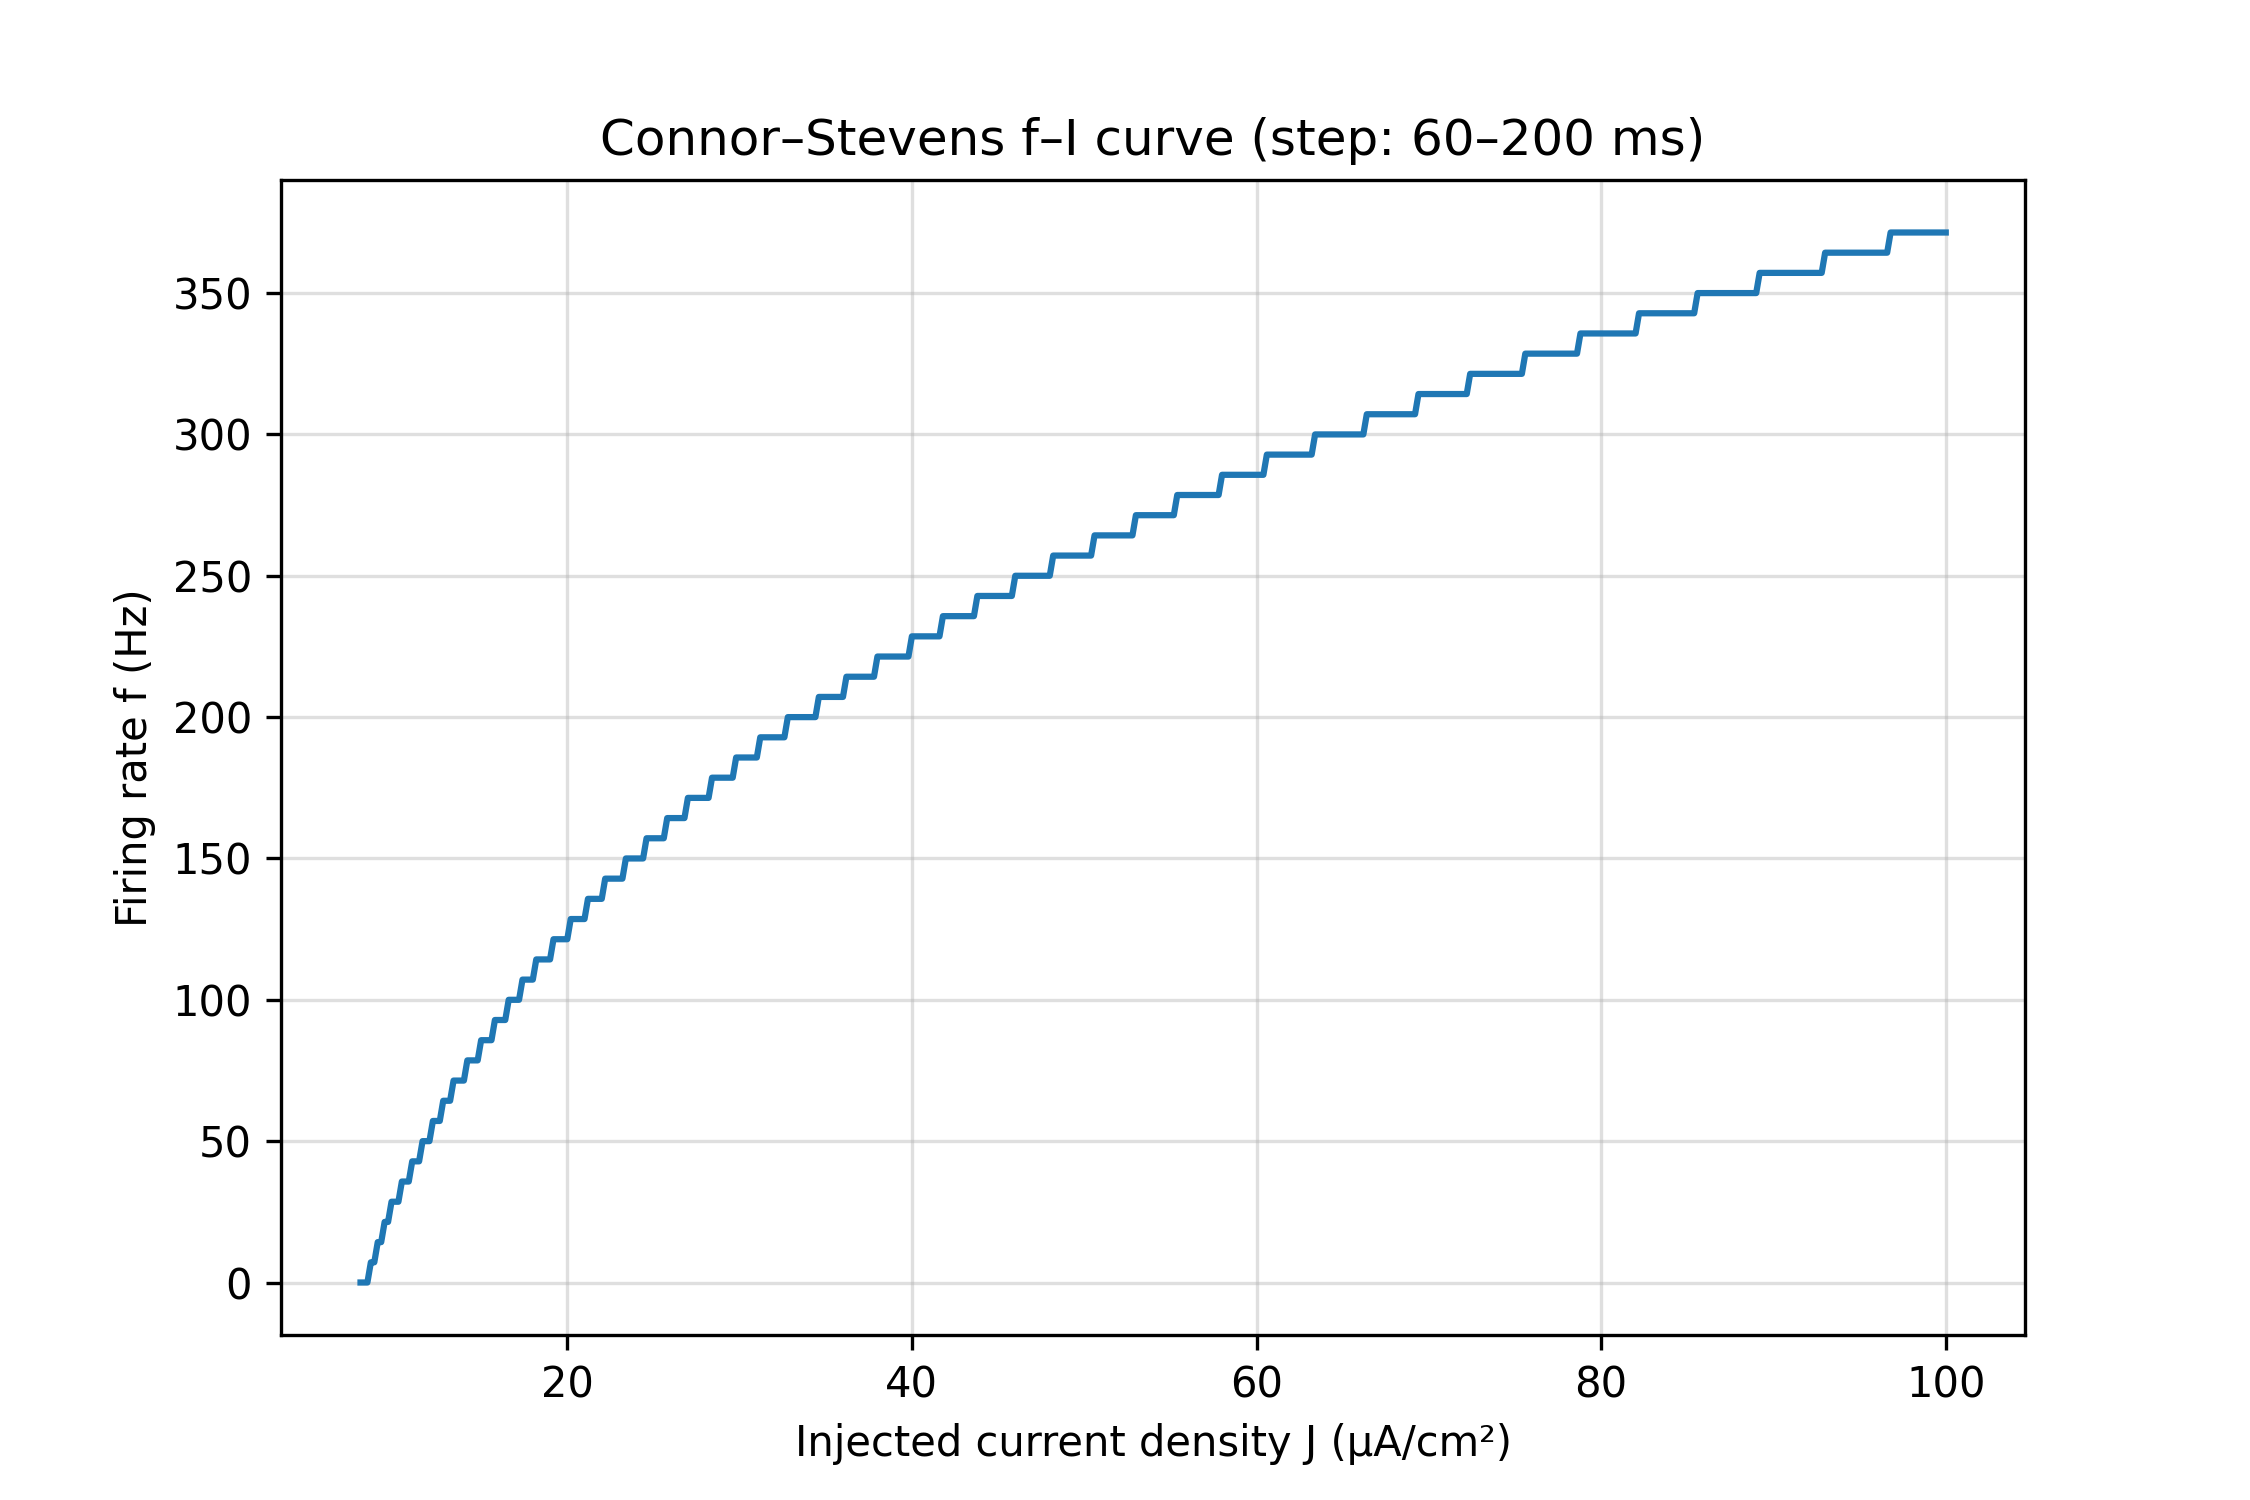
\includegraphics[width=11cm]{../figures/ex_1c.png}	
		\caption{Curva f-I para o modelo de Connor-Stevens.}
	\end{figure}
	
	O formato da curva foi similar ao obtido para Hodgkin-Huxley, porém, os valores de $f$ para um mesmo $V$ foram consideravemente maiores desta vez.\\
	
	\noindent \textbf{(d)} Outra maneira de determinar a taxa de disparos de um neurônio em resposta a uma corrente é calculando o tempo entre o início do estímulo e o primeiro disparo do neurônio (chamado de \textit{latência} do primeiro disparo). A taxa de disparos neste caso é dada pelo inverso da latência do primeiro disparo. Determine a curva f-I para o modelo de Connor-Stevens por esse método para as mesmas correntes usadas no item anterior.
	
	\begin{figure}[H]
		\centering
		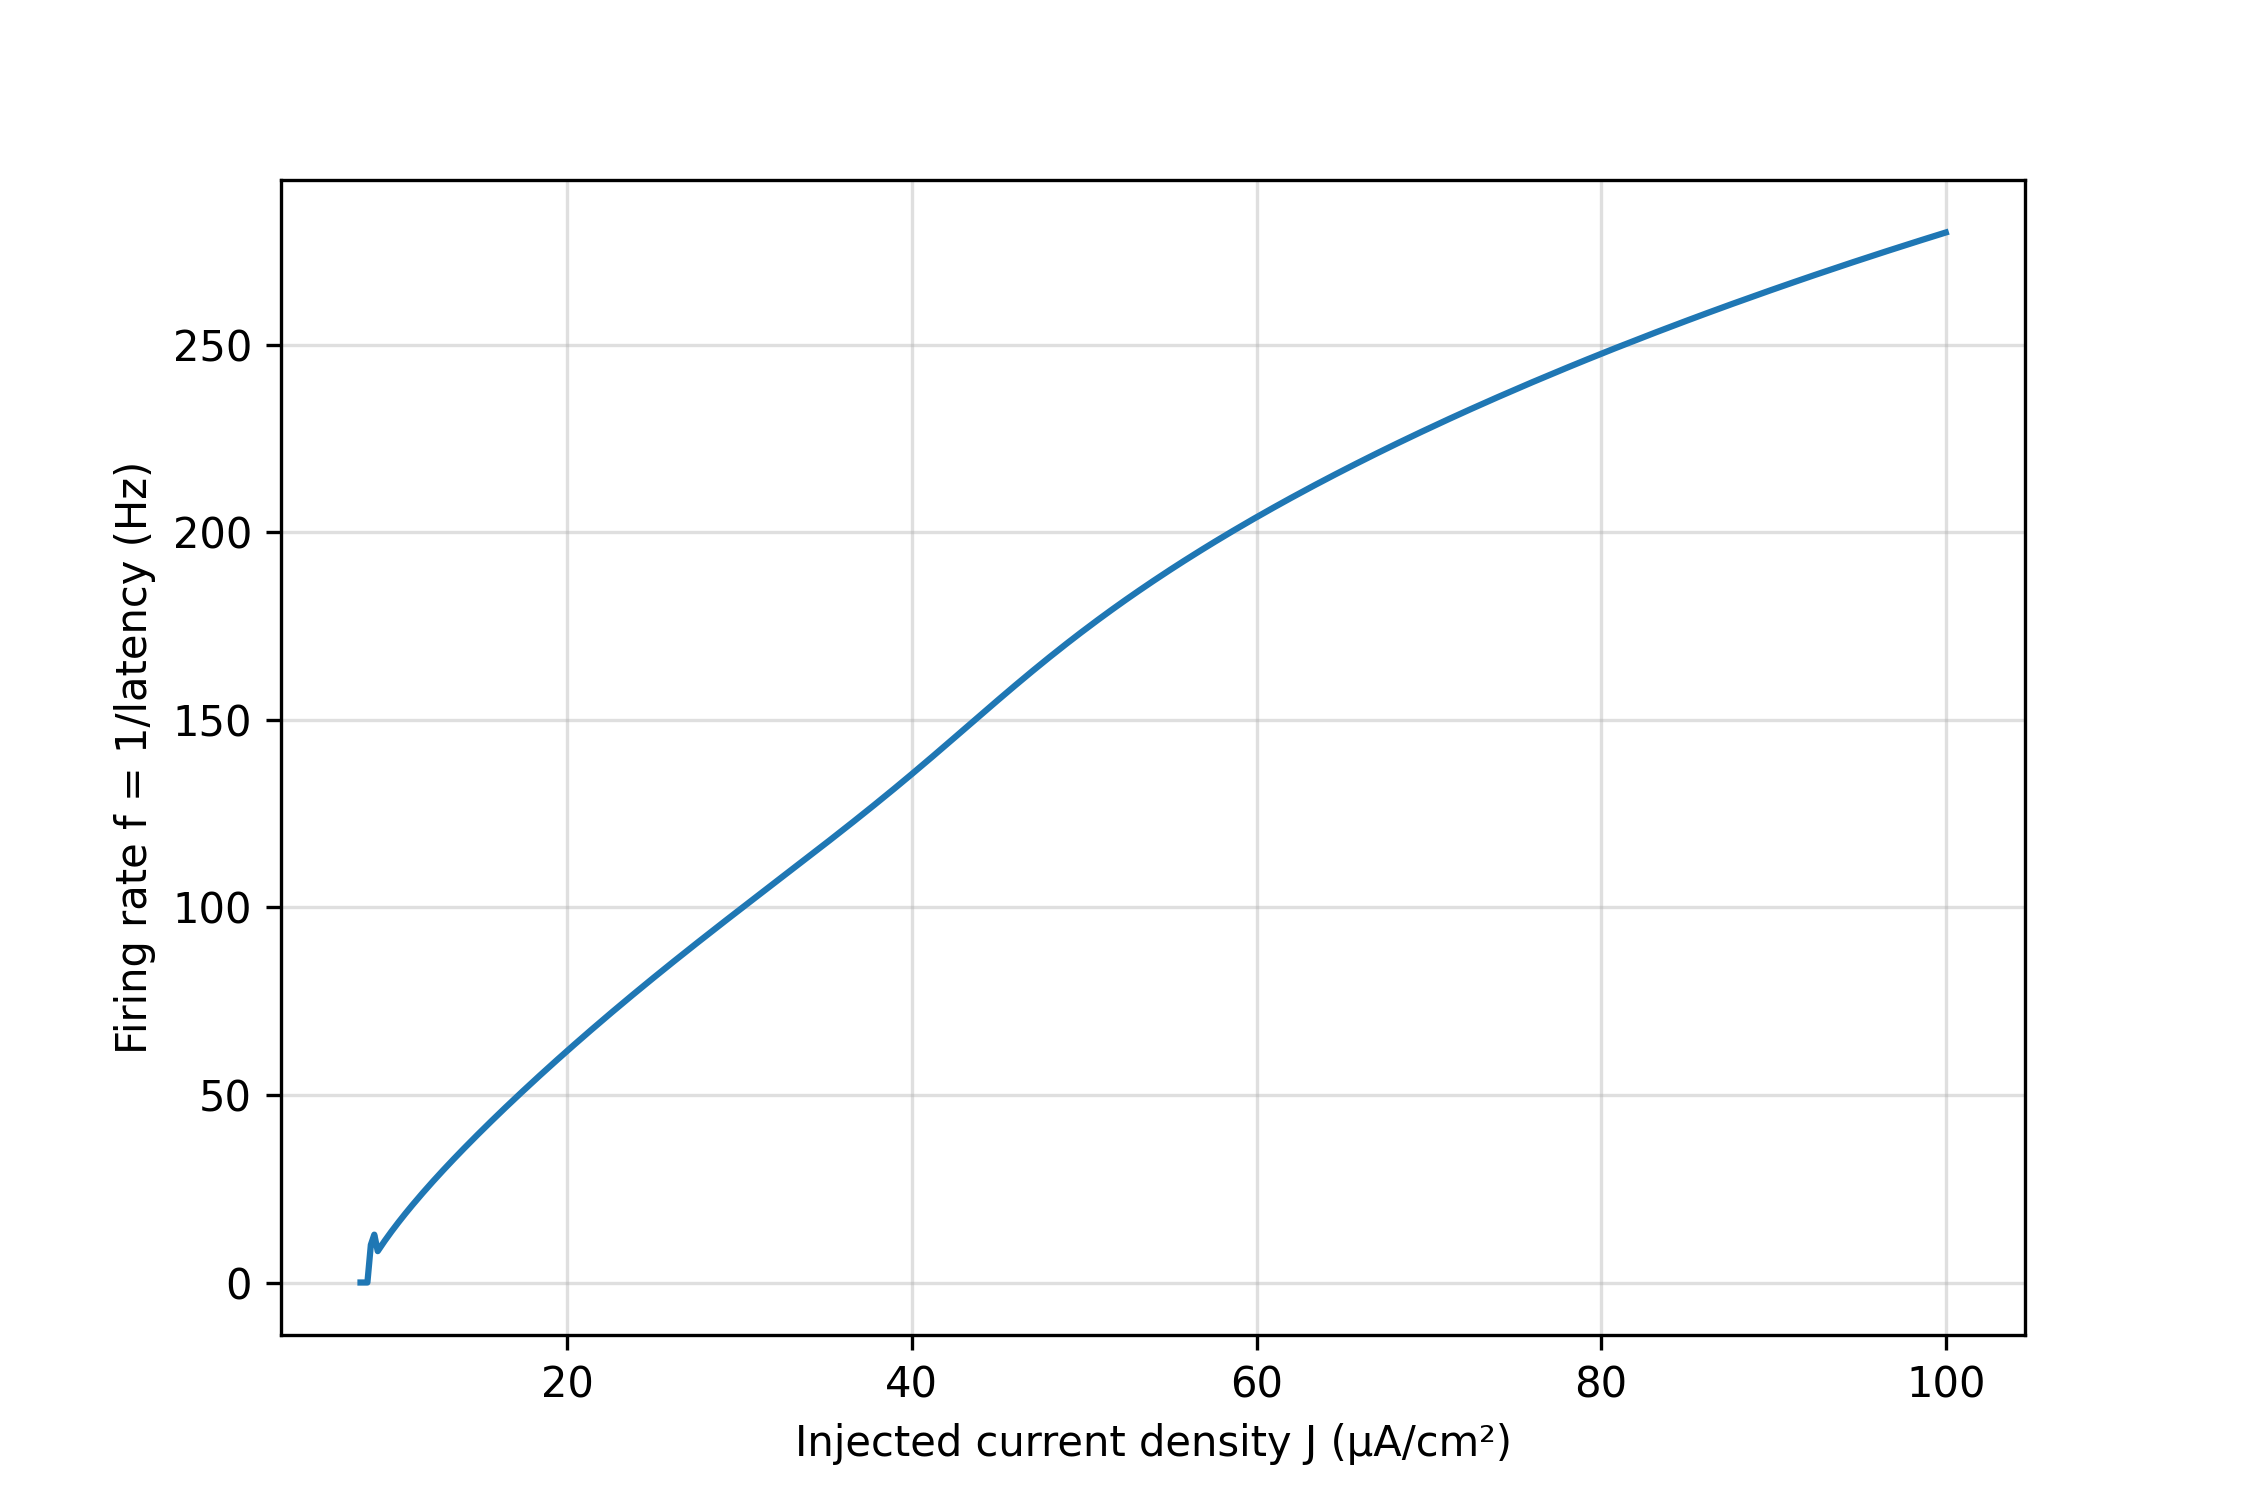
\includegraphics[width=11cm]{../figures/ex_1d.png}	
		\caption{Curva f-I determinada através do tempo de latência do primeiro disparo.}
	\end{figure}
	
	\noindent \textbf{(e)} Em $t = 60 \ \text{ms}$, aplique uma densidade de corrente negativa igual a $J = -50 \ \mu A/\text{cm}^2$ por $5 \ \text{ms}$ (um pulso de corrente negativa) e, em seguida, aplique uma densidade de corrente constante positiva de $J = 20 \ \mu A/\text{cm}^2$ até o fim da simulação. Faça o gráfico de $V$ \textit{versus} $t$ para esse caso.\\
	
	\begin{figure}[H]
	\centering
	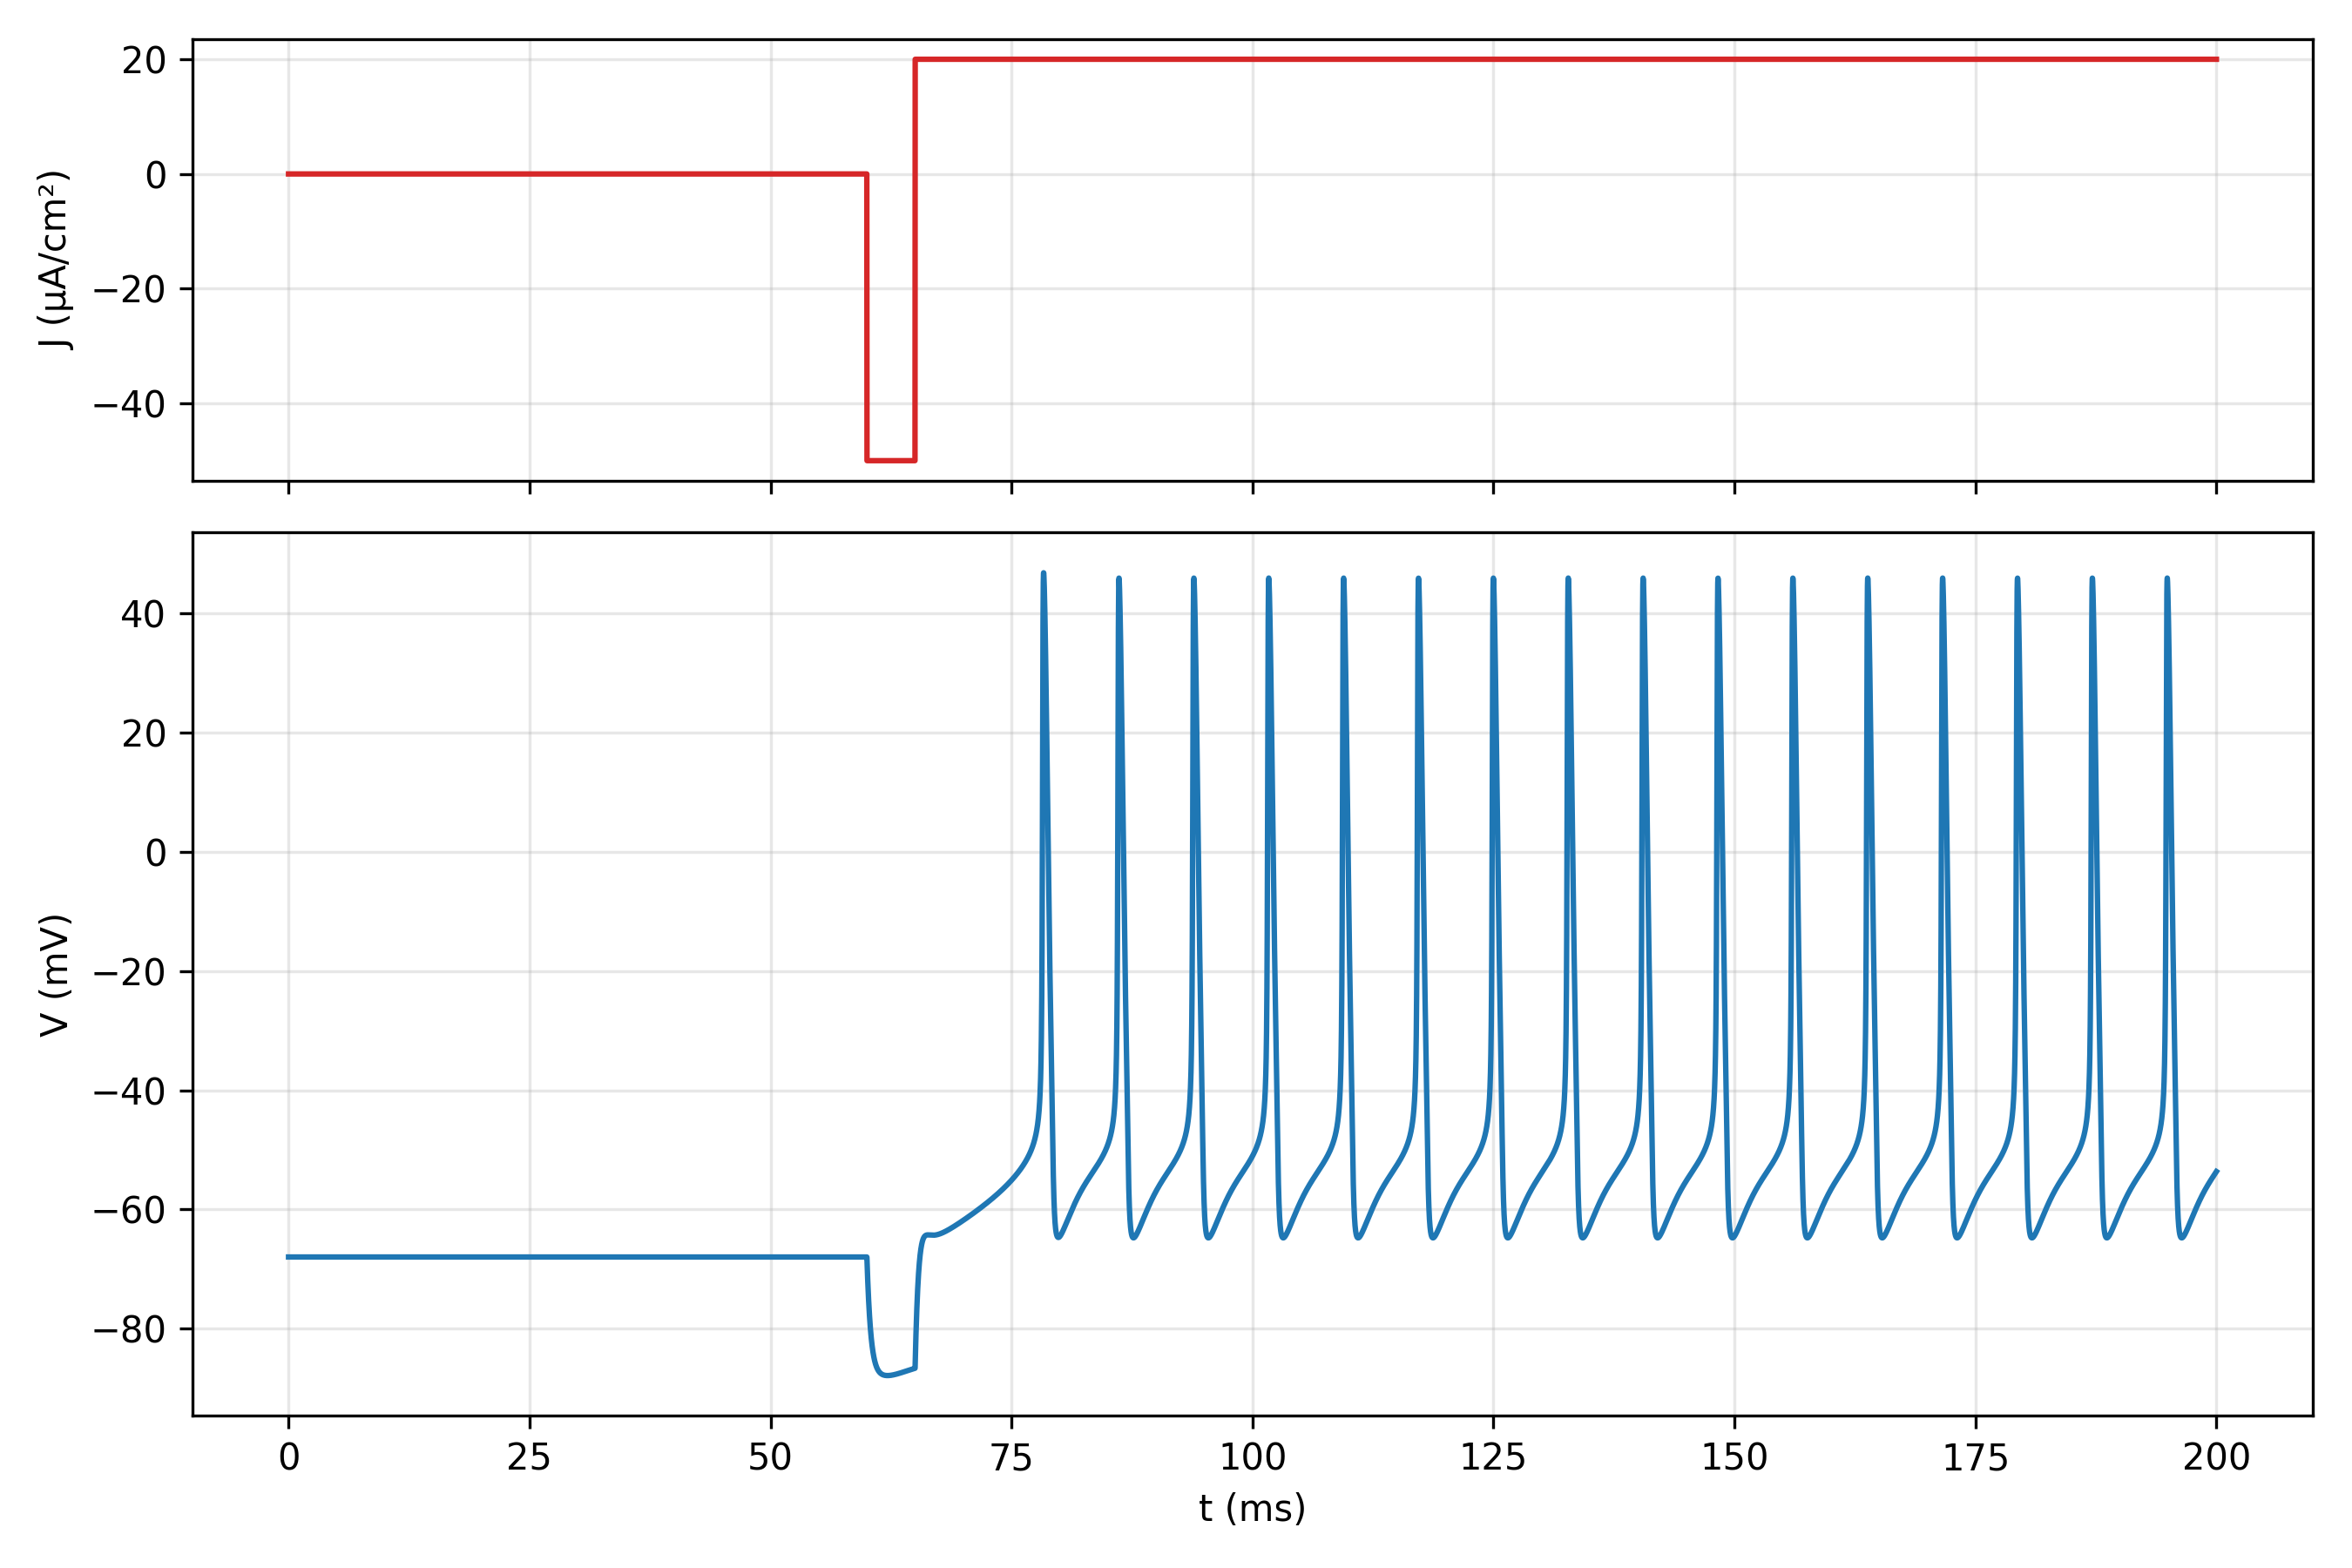
\includegraphics[width=11cm]{../figures/ex_1e.png}	
	\caption{Comportamento de $V$ sob corrente injetada conforme o enunciado.}
	\end{figure}
	
	
	
	\noindent \textbf{(f)} Multiplique o termo do lado direito da equação (6) para $db/dt$ por $0{,}25$ para tornar a inativação da corrente A mais lenta. Injete uma densidade de corrente $J = 15 \ \mu A/\text{cm}^2$ e faça o gráfico de $V$ \textit{versus} $t$. Observe que agora a latência do primeiro disparo torna-se muito longa, mas o intervalo entre disparos é bem pequeno. Explique o motivo disso.\\
	
		\begin{figure}[H]
		\centering
		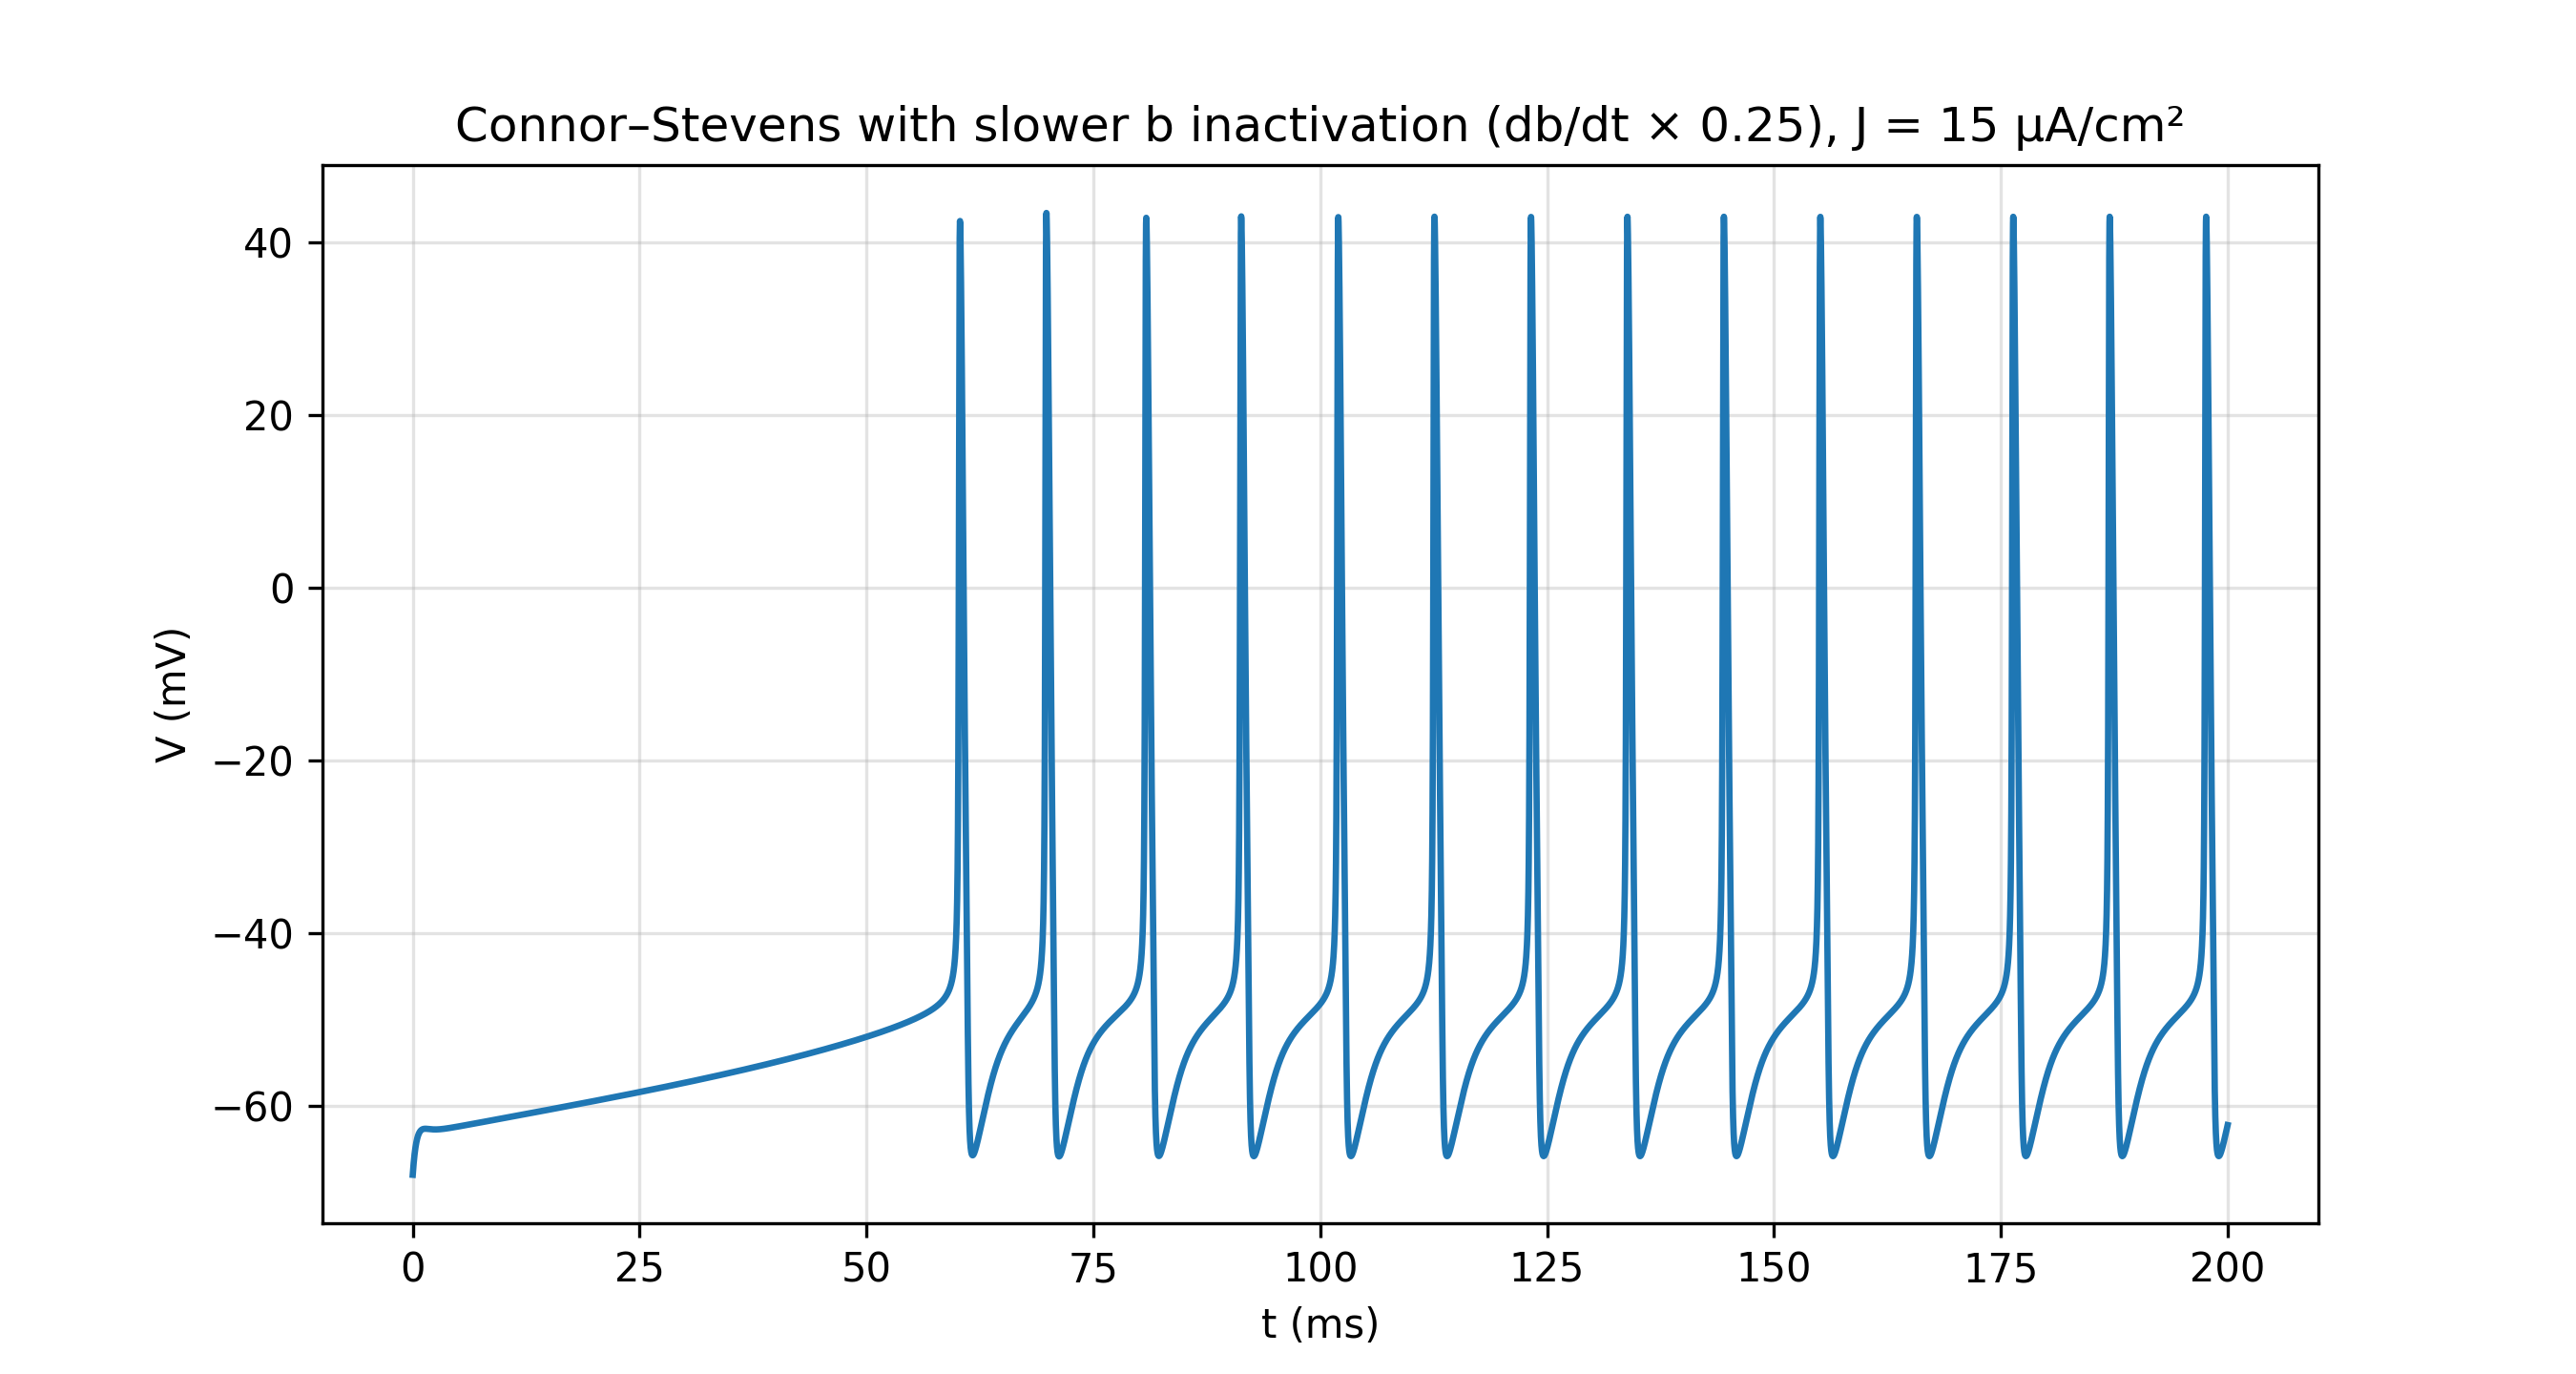
\includegraphics[width=11cm]{../figures/ex_1f.png}	
		\caption{Comportamento de $V$ para inativação lenta da corrente A.}
		\end{figure}
	
	A latência do primeiro disparo é muito maior neste caso pois a corrente A se opõe à despolarização, e com sua inativação mais lenta, ela persiste por mais tempo dificultando o inicio do potencial de ação.\\\\
	
	
	
	\noindent \textbf{Questão 2. Corrente de cálcio de tipo T.}\\
	
	\noindent \textbf{(a)} Faça um programa que simule o modelo de neurônio de relé talâmico por um período de $750 \ \text{ms}$. Faça o programa de tal forma que você tenha que dar a ele duas entradas: uma corrente de base e um degrau de corrente. A corrente injetada $I_{\text{inj}}$ na equação (7) deve receber o valor da corrente de base de $t = 0$ a $t = 250 \ \text{ms}$. Em $t = 250 \ \text{ms}$ a corrente injetada $I_{\text{inj}}$ deve ser incrementada pelo valor do degrau de corrente e mantida assim até $t = 500 \ \text{ms}$. De $t = 500 \ \text{ms}$ a $t = 750 \ \text{ms}$, a corrente injetada $I_{\text{inj}}$ deve voltar ao valor da corrente de base. Faça seu programa produzir gráficos de $V, \ n, \ h \ e \ h_T$ \textit{versus} $t$ pelo tempo de simulação do experimento.\\
	
	\begin{figure}[H]
		\centering
		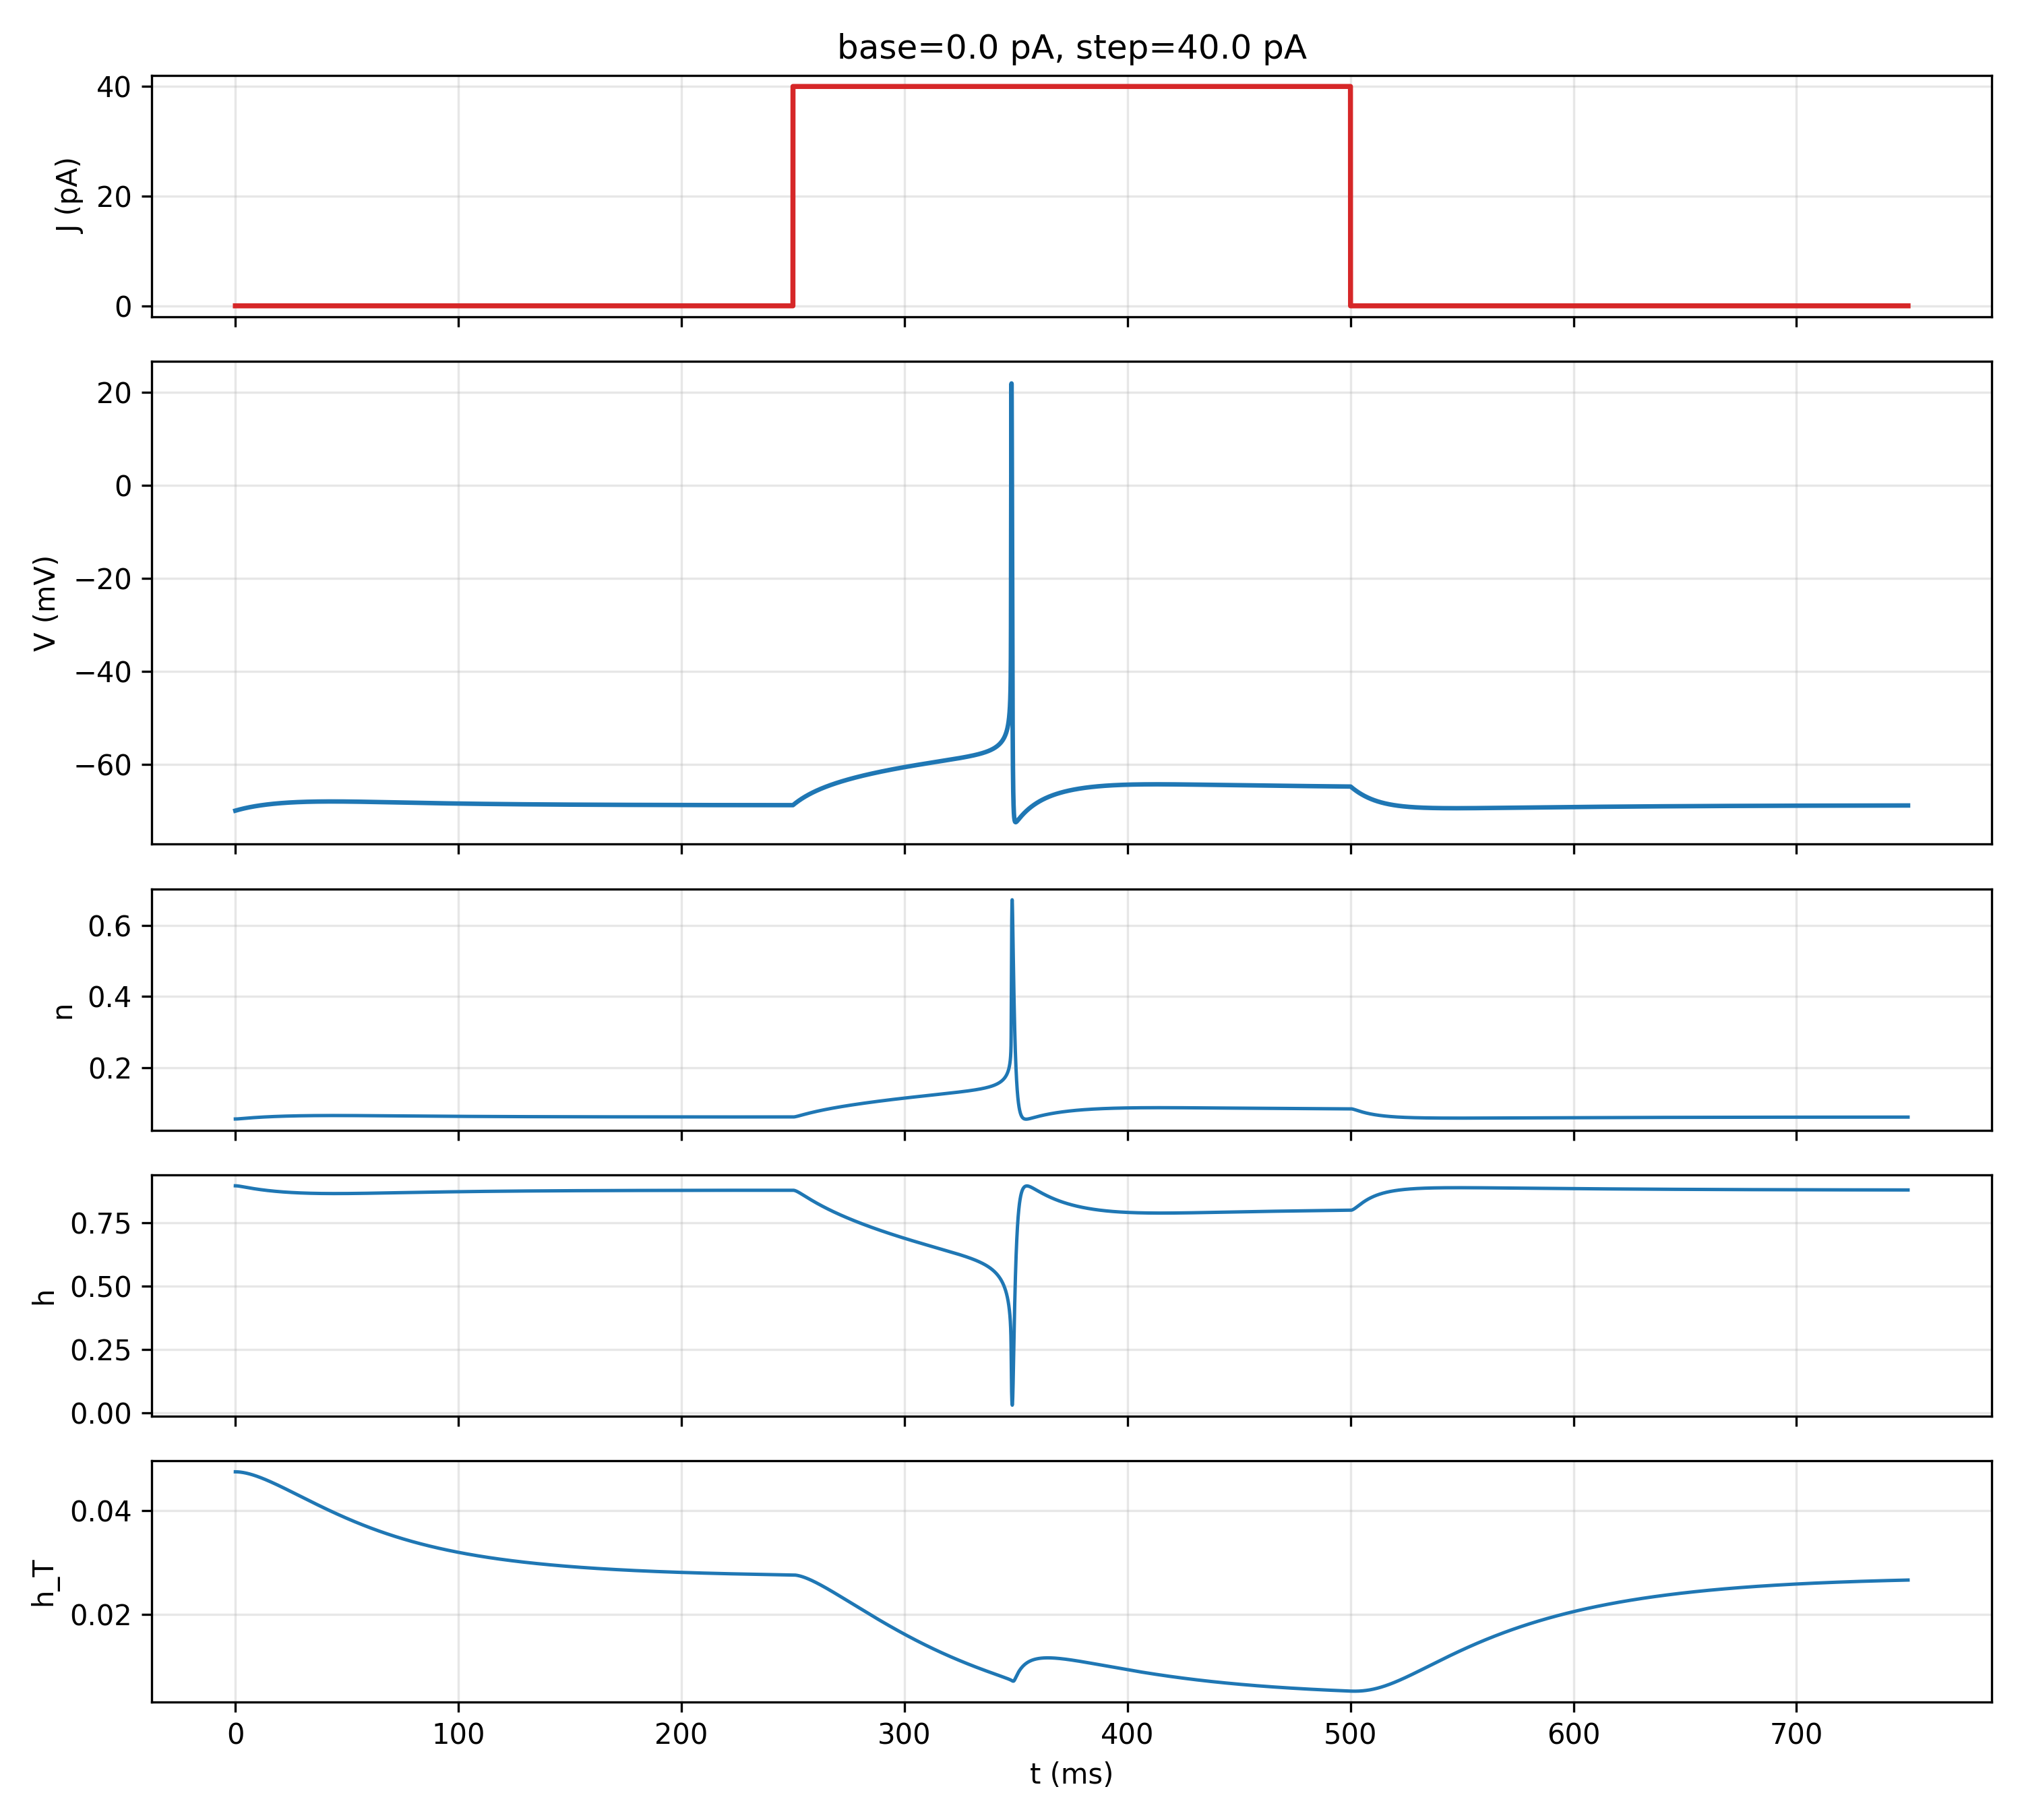
\includegraphics[width=11cm]{../figures/ex_2a.png}	
		\caption{Comportamento do modelo relé talâmico para degrau de corrente pedido no enunciado.}
	\end{figure}
	
	\noindent \textbf{(b)} Faça o seu programa gerar um laço (\textit{loop}) pelos valores da corrente de base (entre $-200 \ \text{pA}$ e $+200 \ \text{pA}$) e pelos valores do degrau de corrente (entre $0$ e $+100 \ \text{pA}$). A escolha dos valores usados dentro desses intervalos fica à sua escolha. Para cada par desses valores (corrente de base e degrau de corrente), calcule o número de disparos emitidos durante a aplicação do degrau de corrente e, caso dois ou mais disparos sejam emitidos, calcule o intervalo mínimo entre disparos. Usando alguma ferramenta para criar gráficos tri-dimensionais, produza dois gráficos tendo a corrente de base no eixo $x$ e o degrau de corrente no eixo $y$. O primeiro gráfico deve mostrar o número de disparos durante a aplicação do degrau de corrente e o segundo gráfico deve mostrar o intervalo mínimo entre disparos. Analise seus resultados e forneça alguns gráficos das variáveis $V, \ n, \ h \ e \ h_T$ para cada tipo \textit{qualitativamente} distinto de comportamento observado.
	
	
	\begin{figure}[H]
	\centering
	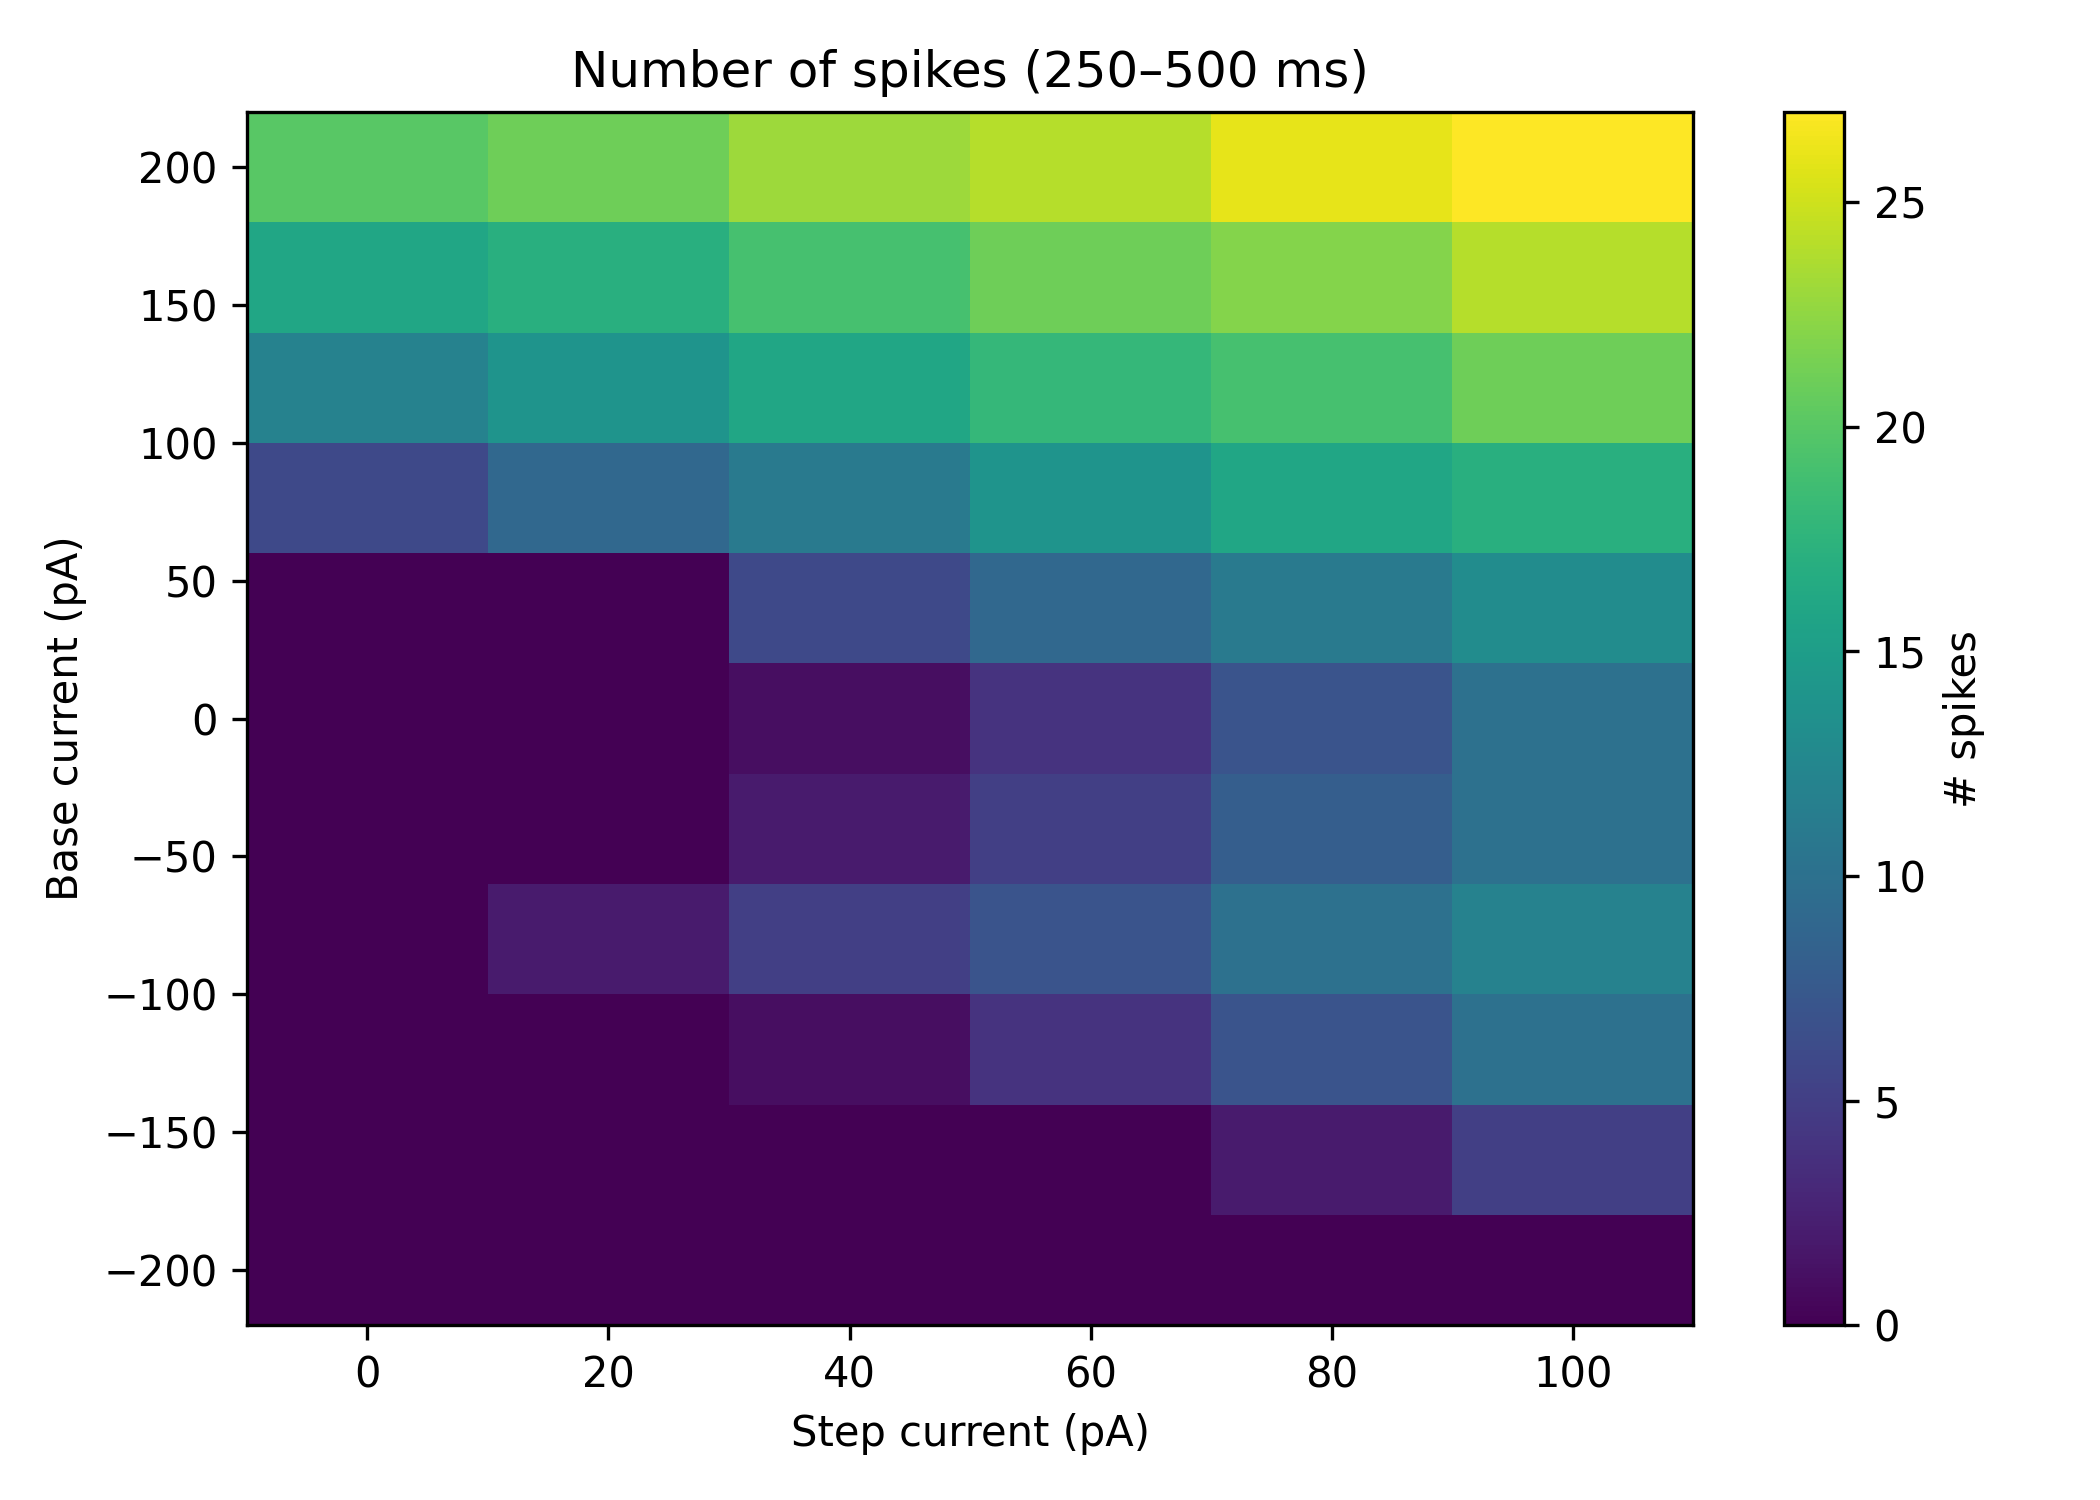
\includegraphics[width=10cm]{../figures/ex_2b_spikecount_heatmap.png}	
	\caption{Mapa de calor da contagem de disparos por par (corrente de base, degrau de corrente).}
	\end{figure}
	\begin{figure}[H]
		\centering
		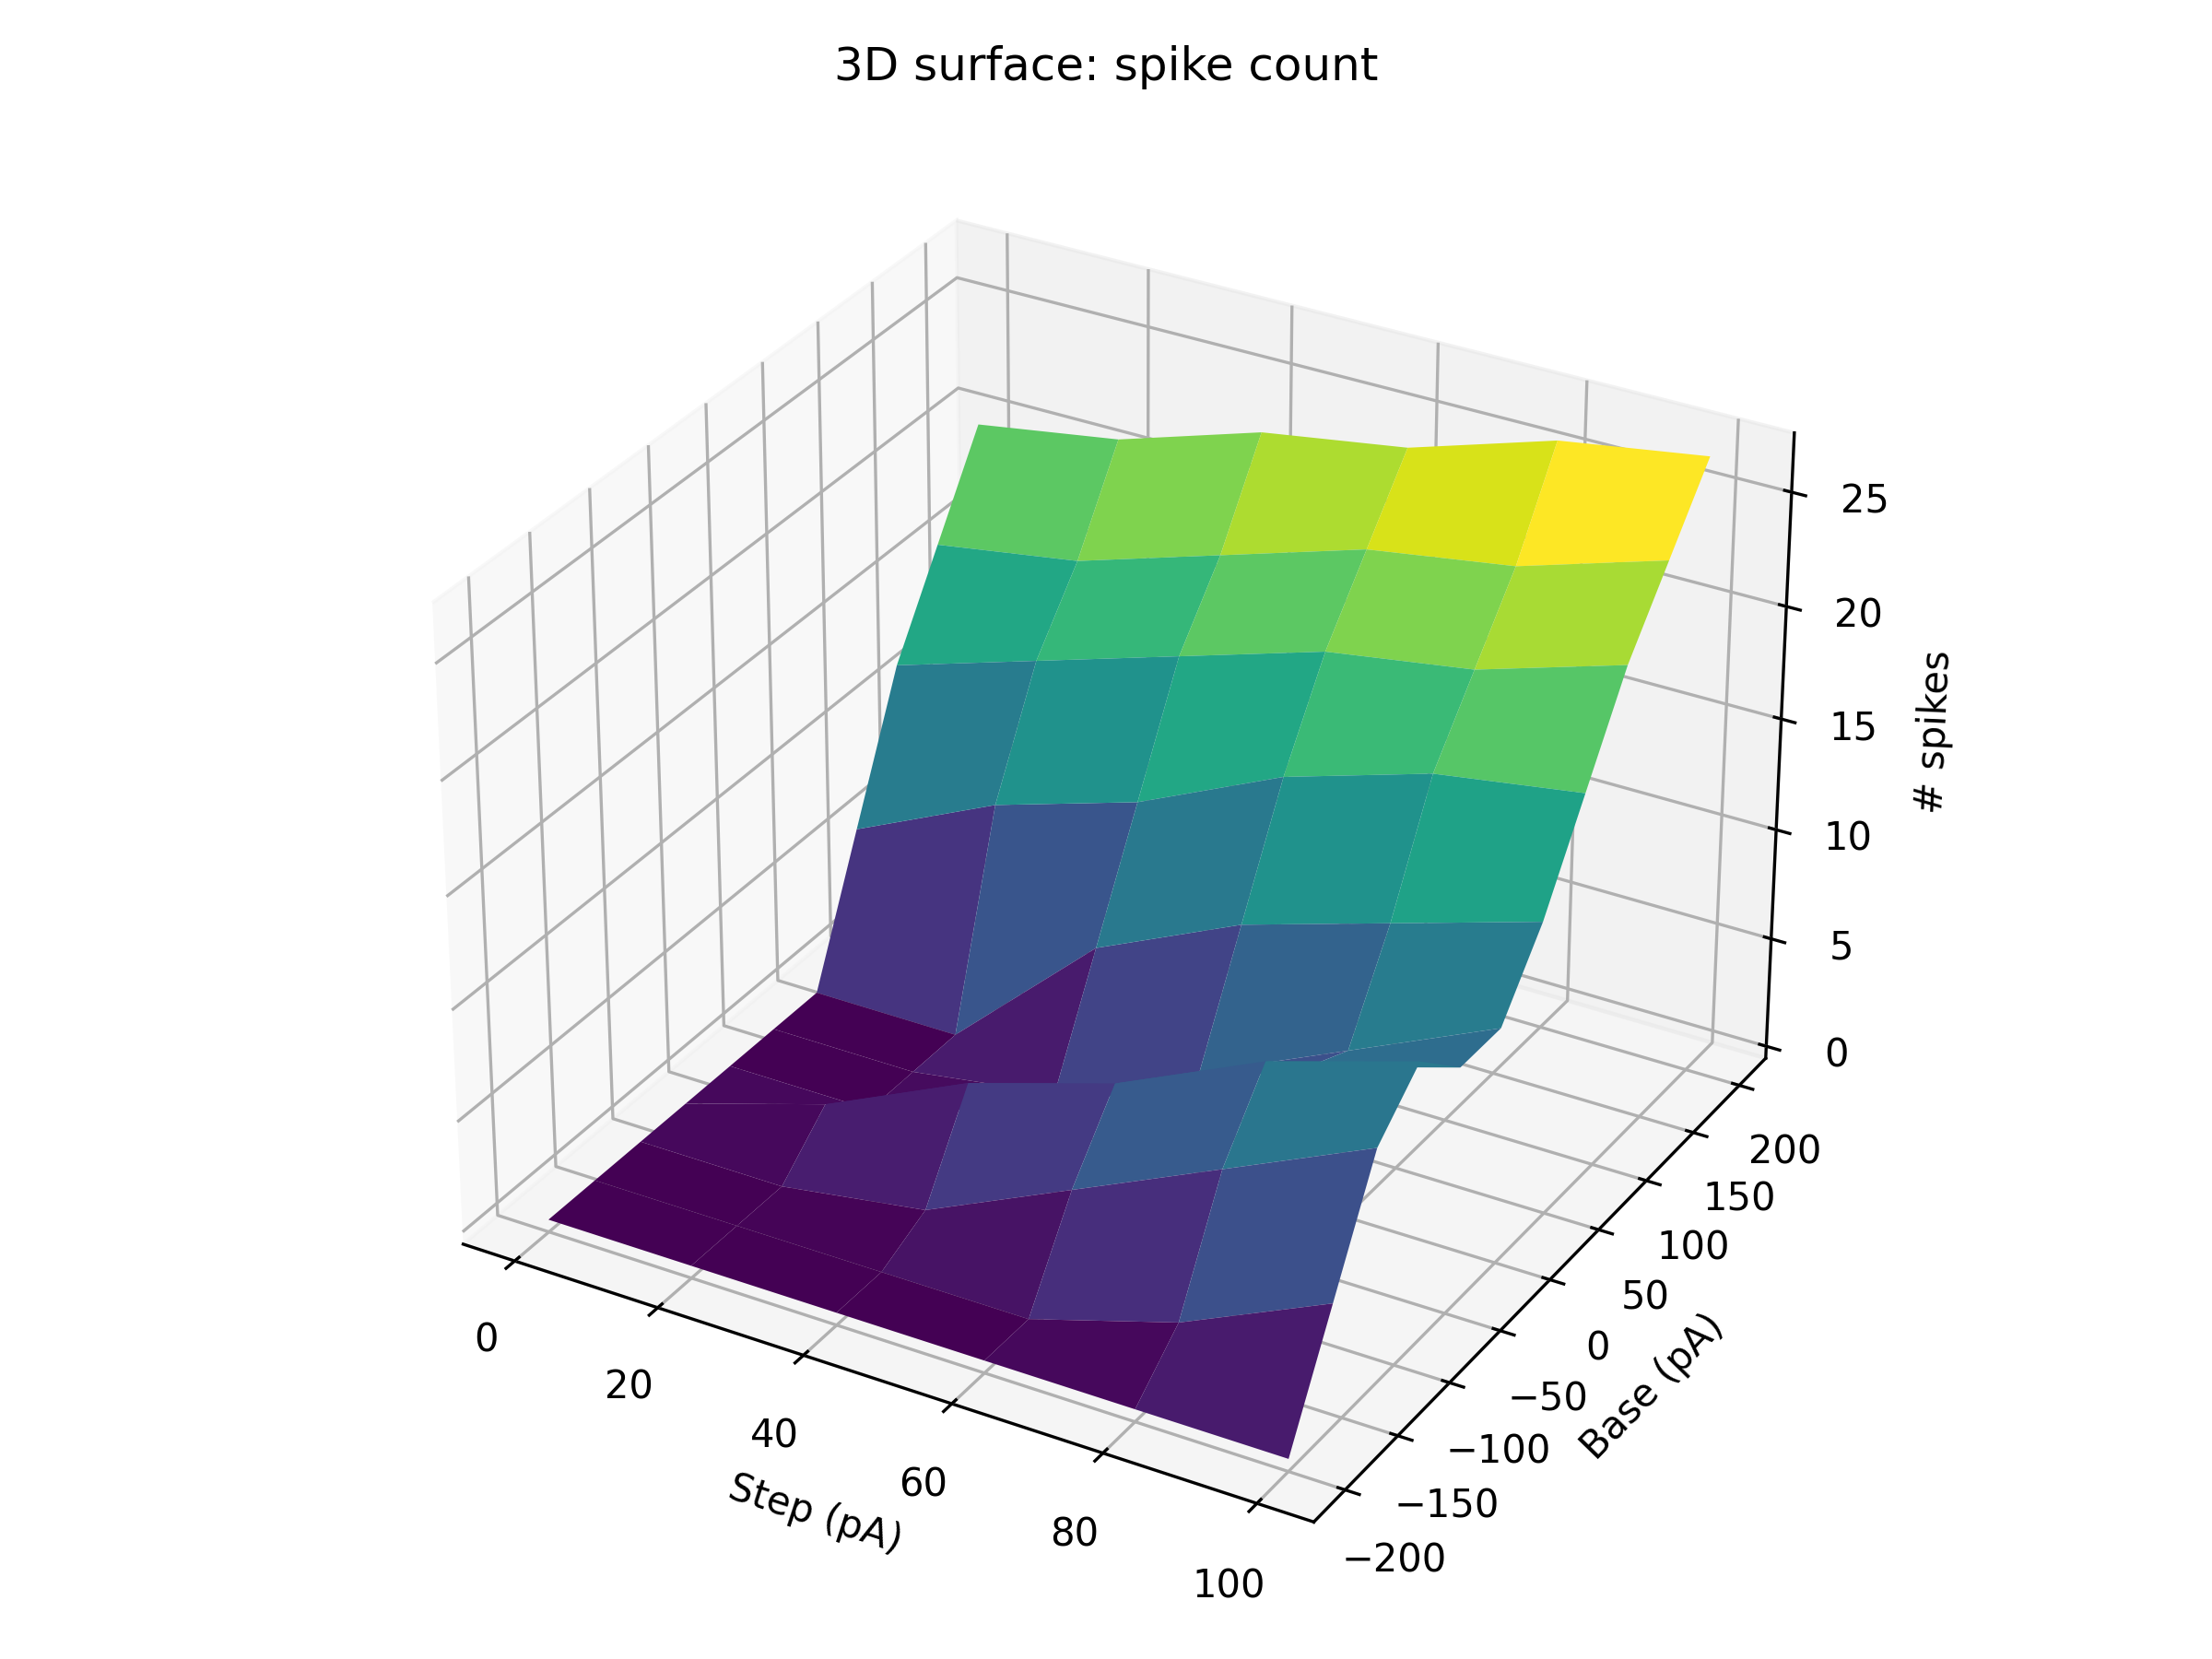
\includegraphics[width=10cm]{../figures/ex_2b_spikecount_surface.png}	
		\caption{Superfície da contagem de disparos por par (corrente de base, degrau de corrente).}
	\end{figure}
	\begin{figure}[H]
	\centering
	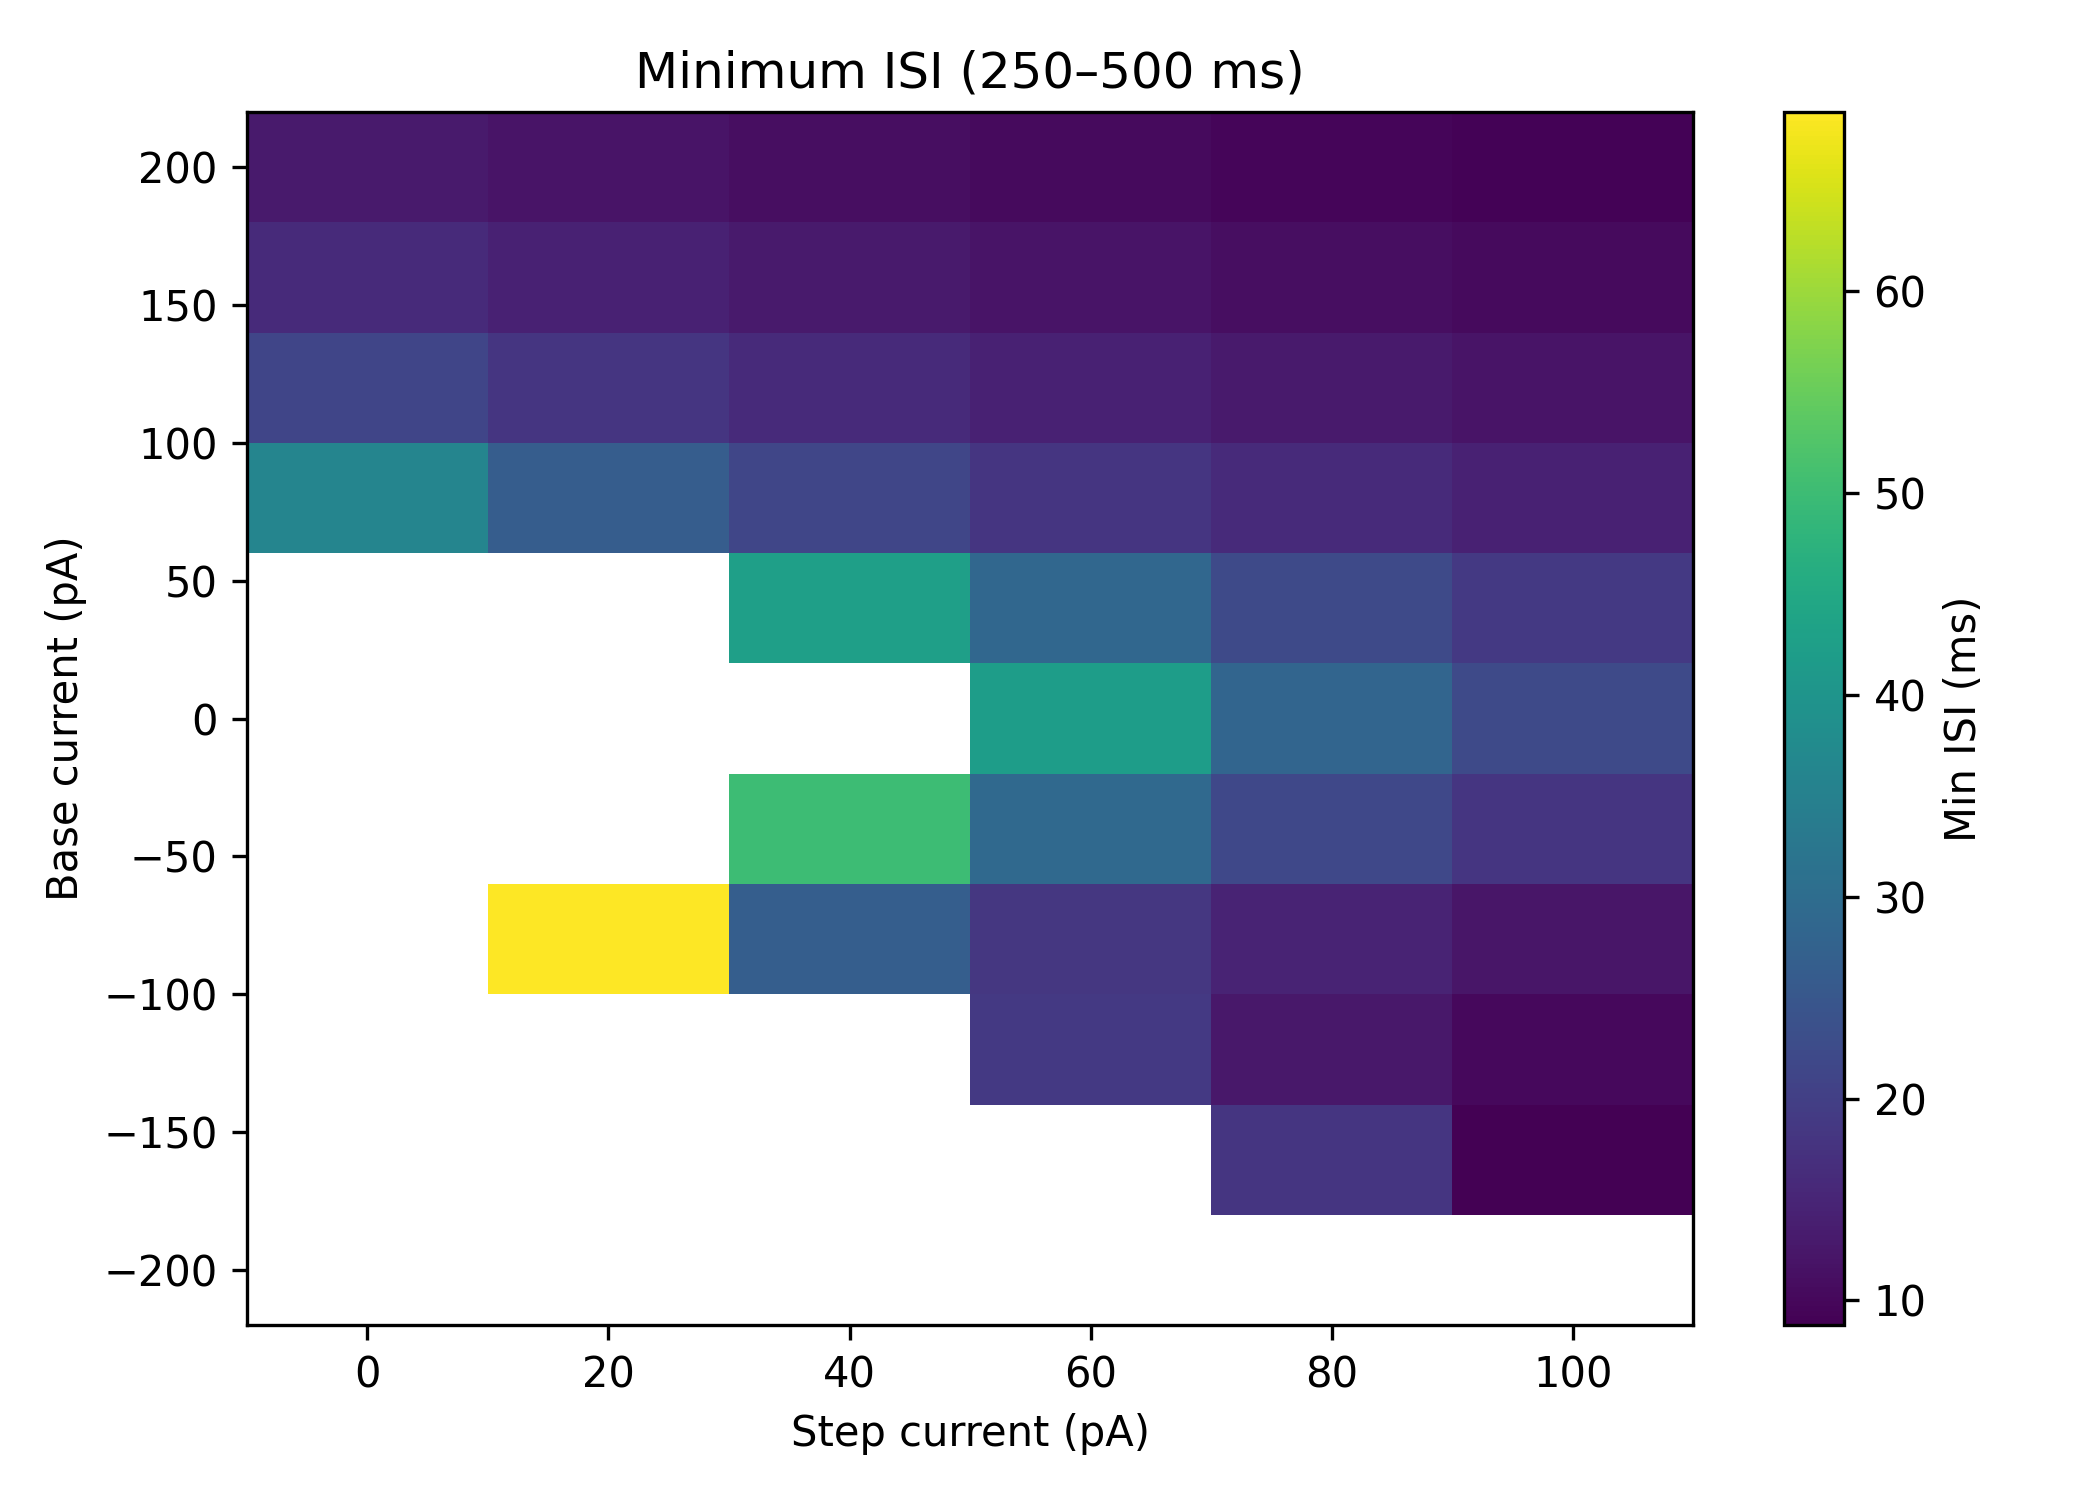
\includegraphics[width=10cm]{../figures/ex_2b_minISI_heatmap.png}	
	\caption{Mapa de calor no intervalo mínimo entre disparos por par (corrente de base, degrau de corrente).}
	\end{figure}
	\begin{figure}[H]
		\centering
		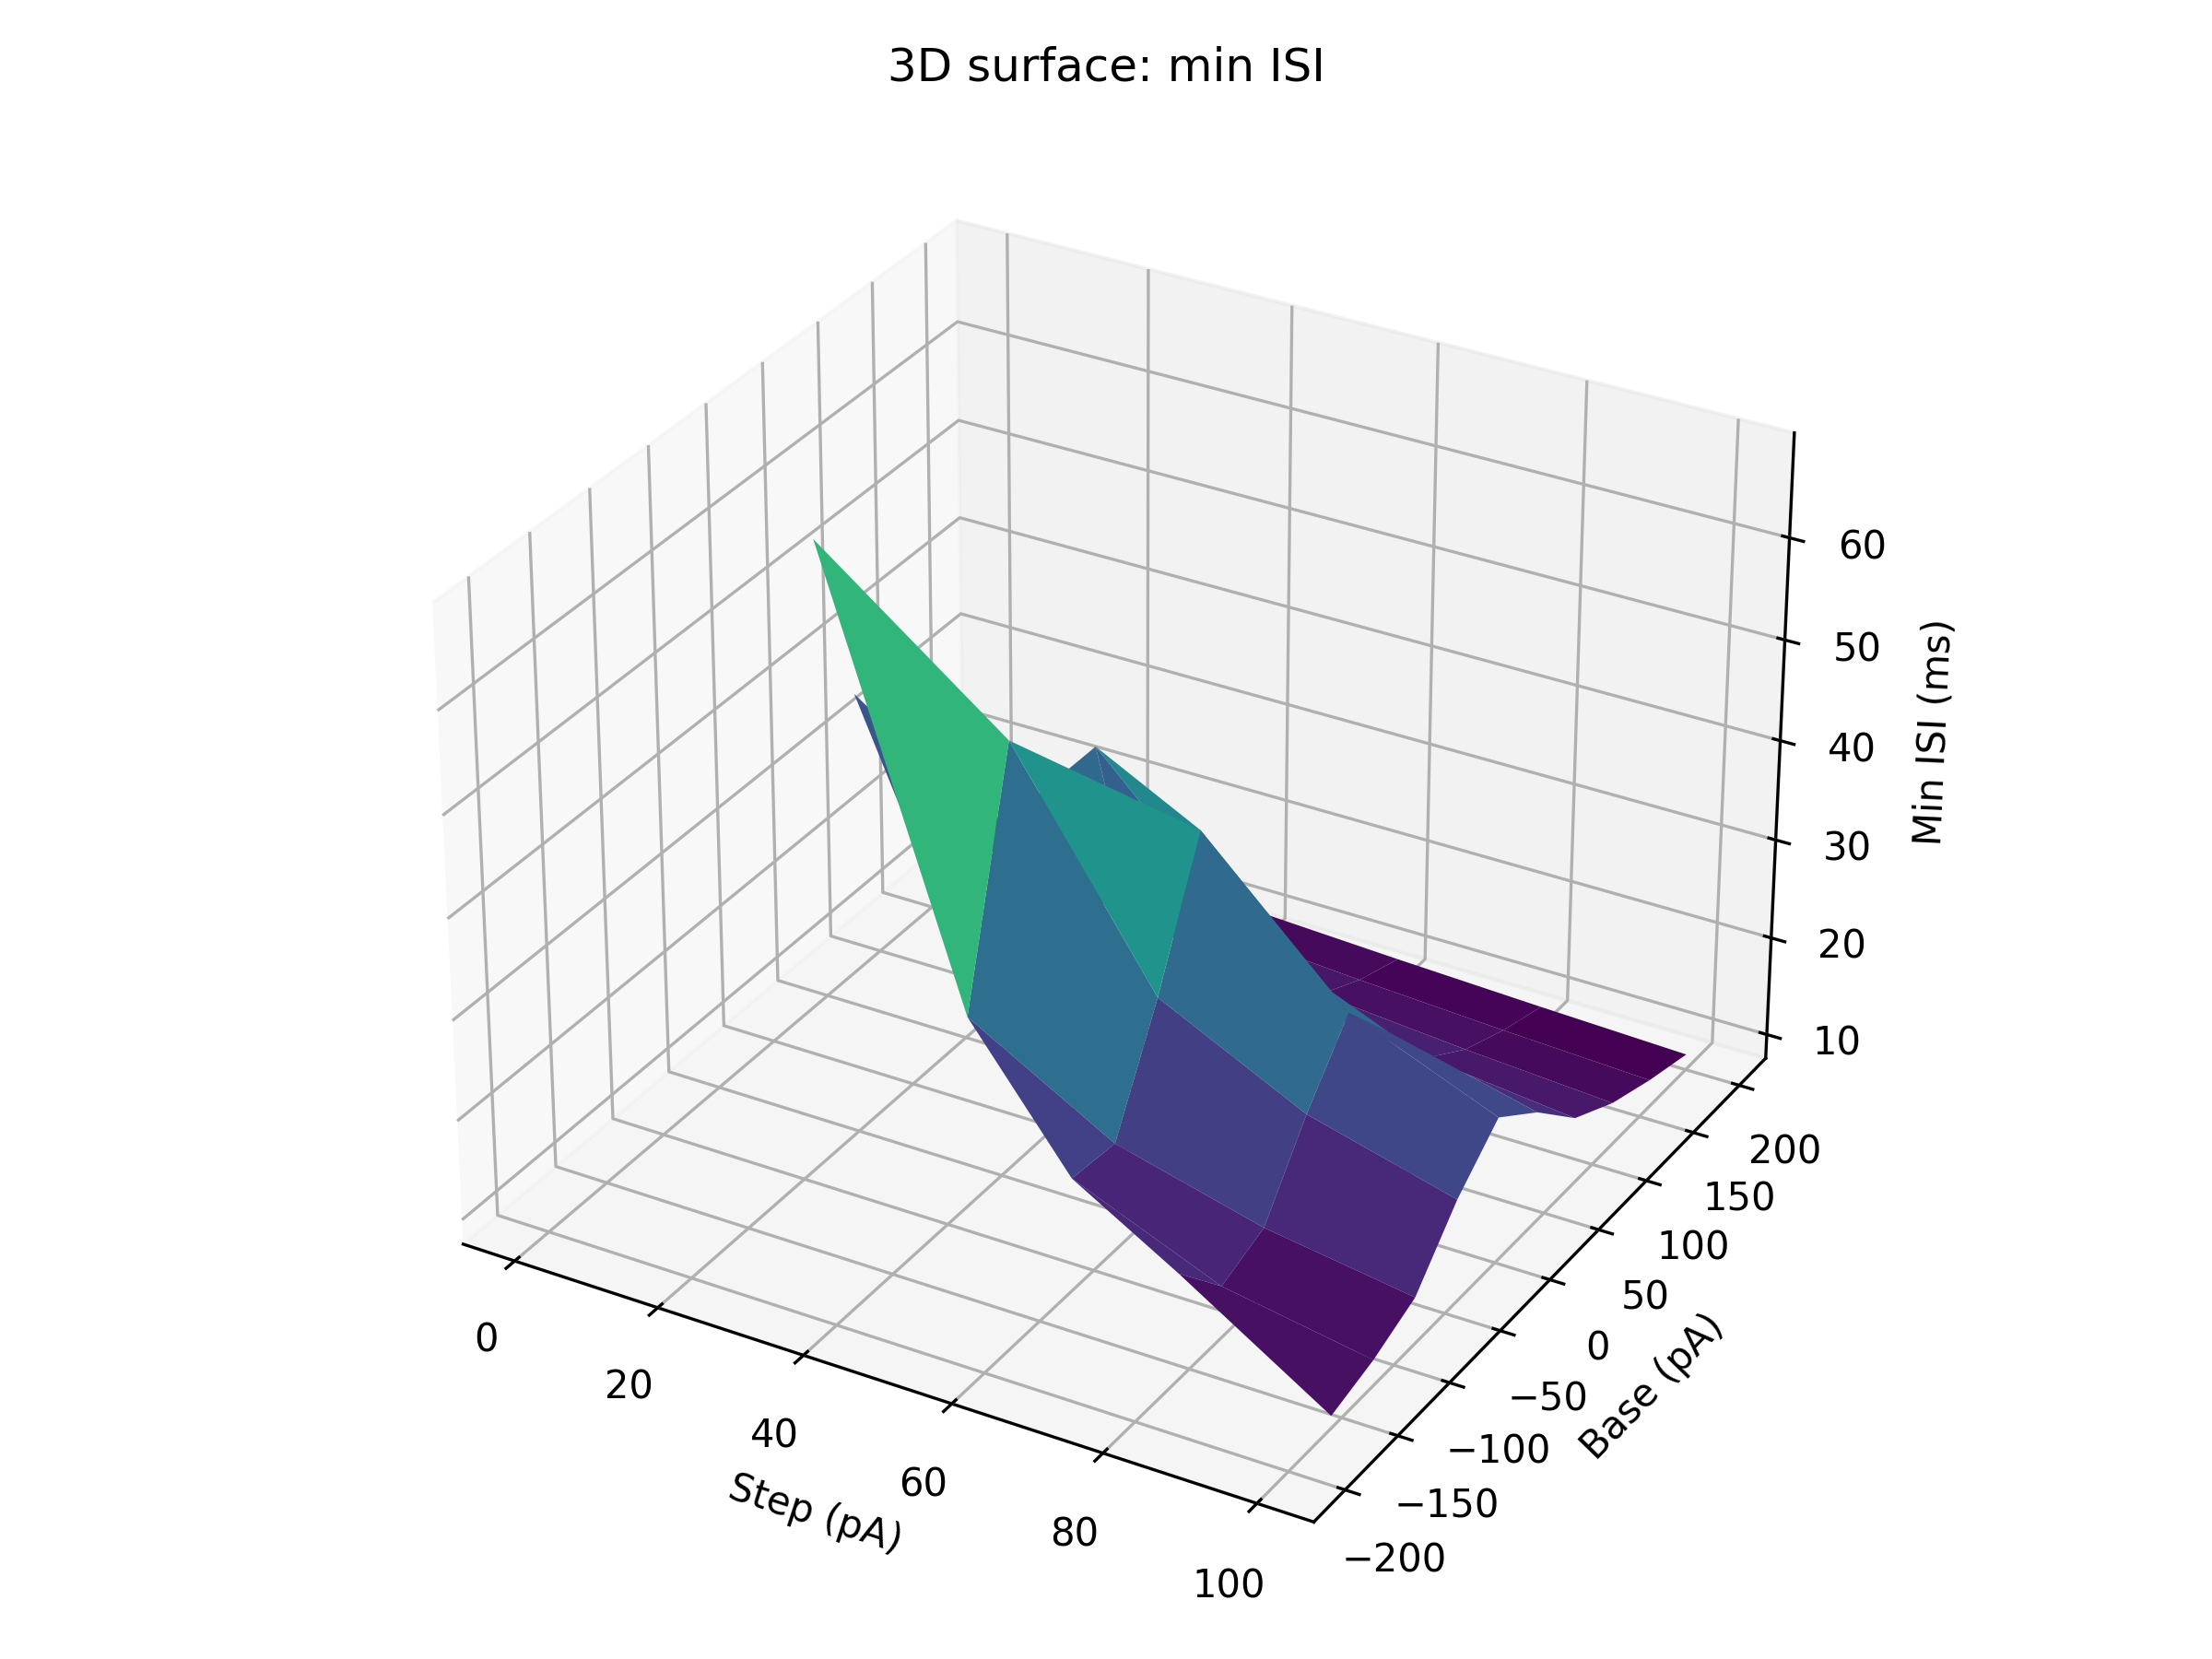
\includegraphics[width=10cm]{../figures/ex_2b_minISI_surface.png}	
		\caption{Superfície no intervalo mínimo entre disparos por par (corrente de base, degrau de corrente).}
	\end{figure}
	
	É possível notar que o número de disparos cresce justamente com a corrente de base e com o degrau de corrente, enquanto que o intervalo mínimo entre disparos obedece a relação contrária: quanto maior a corrente base ou degrau, menor é o intervalo mínimo. É um resultado intuitivo pois, com correntes maiores, maior é o estimulo no neurônio, e mais disparos existem. Por outro lado, quanto mais disparos existem num mesmo intervalo de tempo, menor deve ser o intervalo entre os disparos.
	
	Abaixo estão alguns exemplos de comportamento qualitativamente distintos.
	
	\begin{figure}[H]
		\centering
		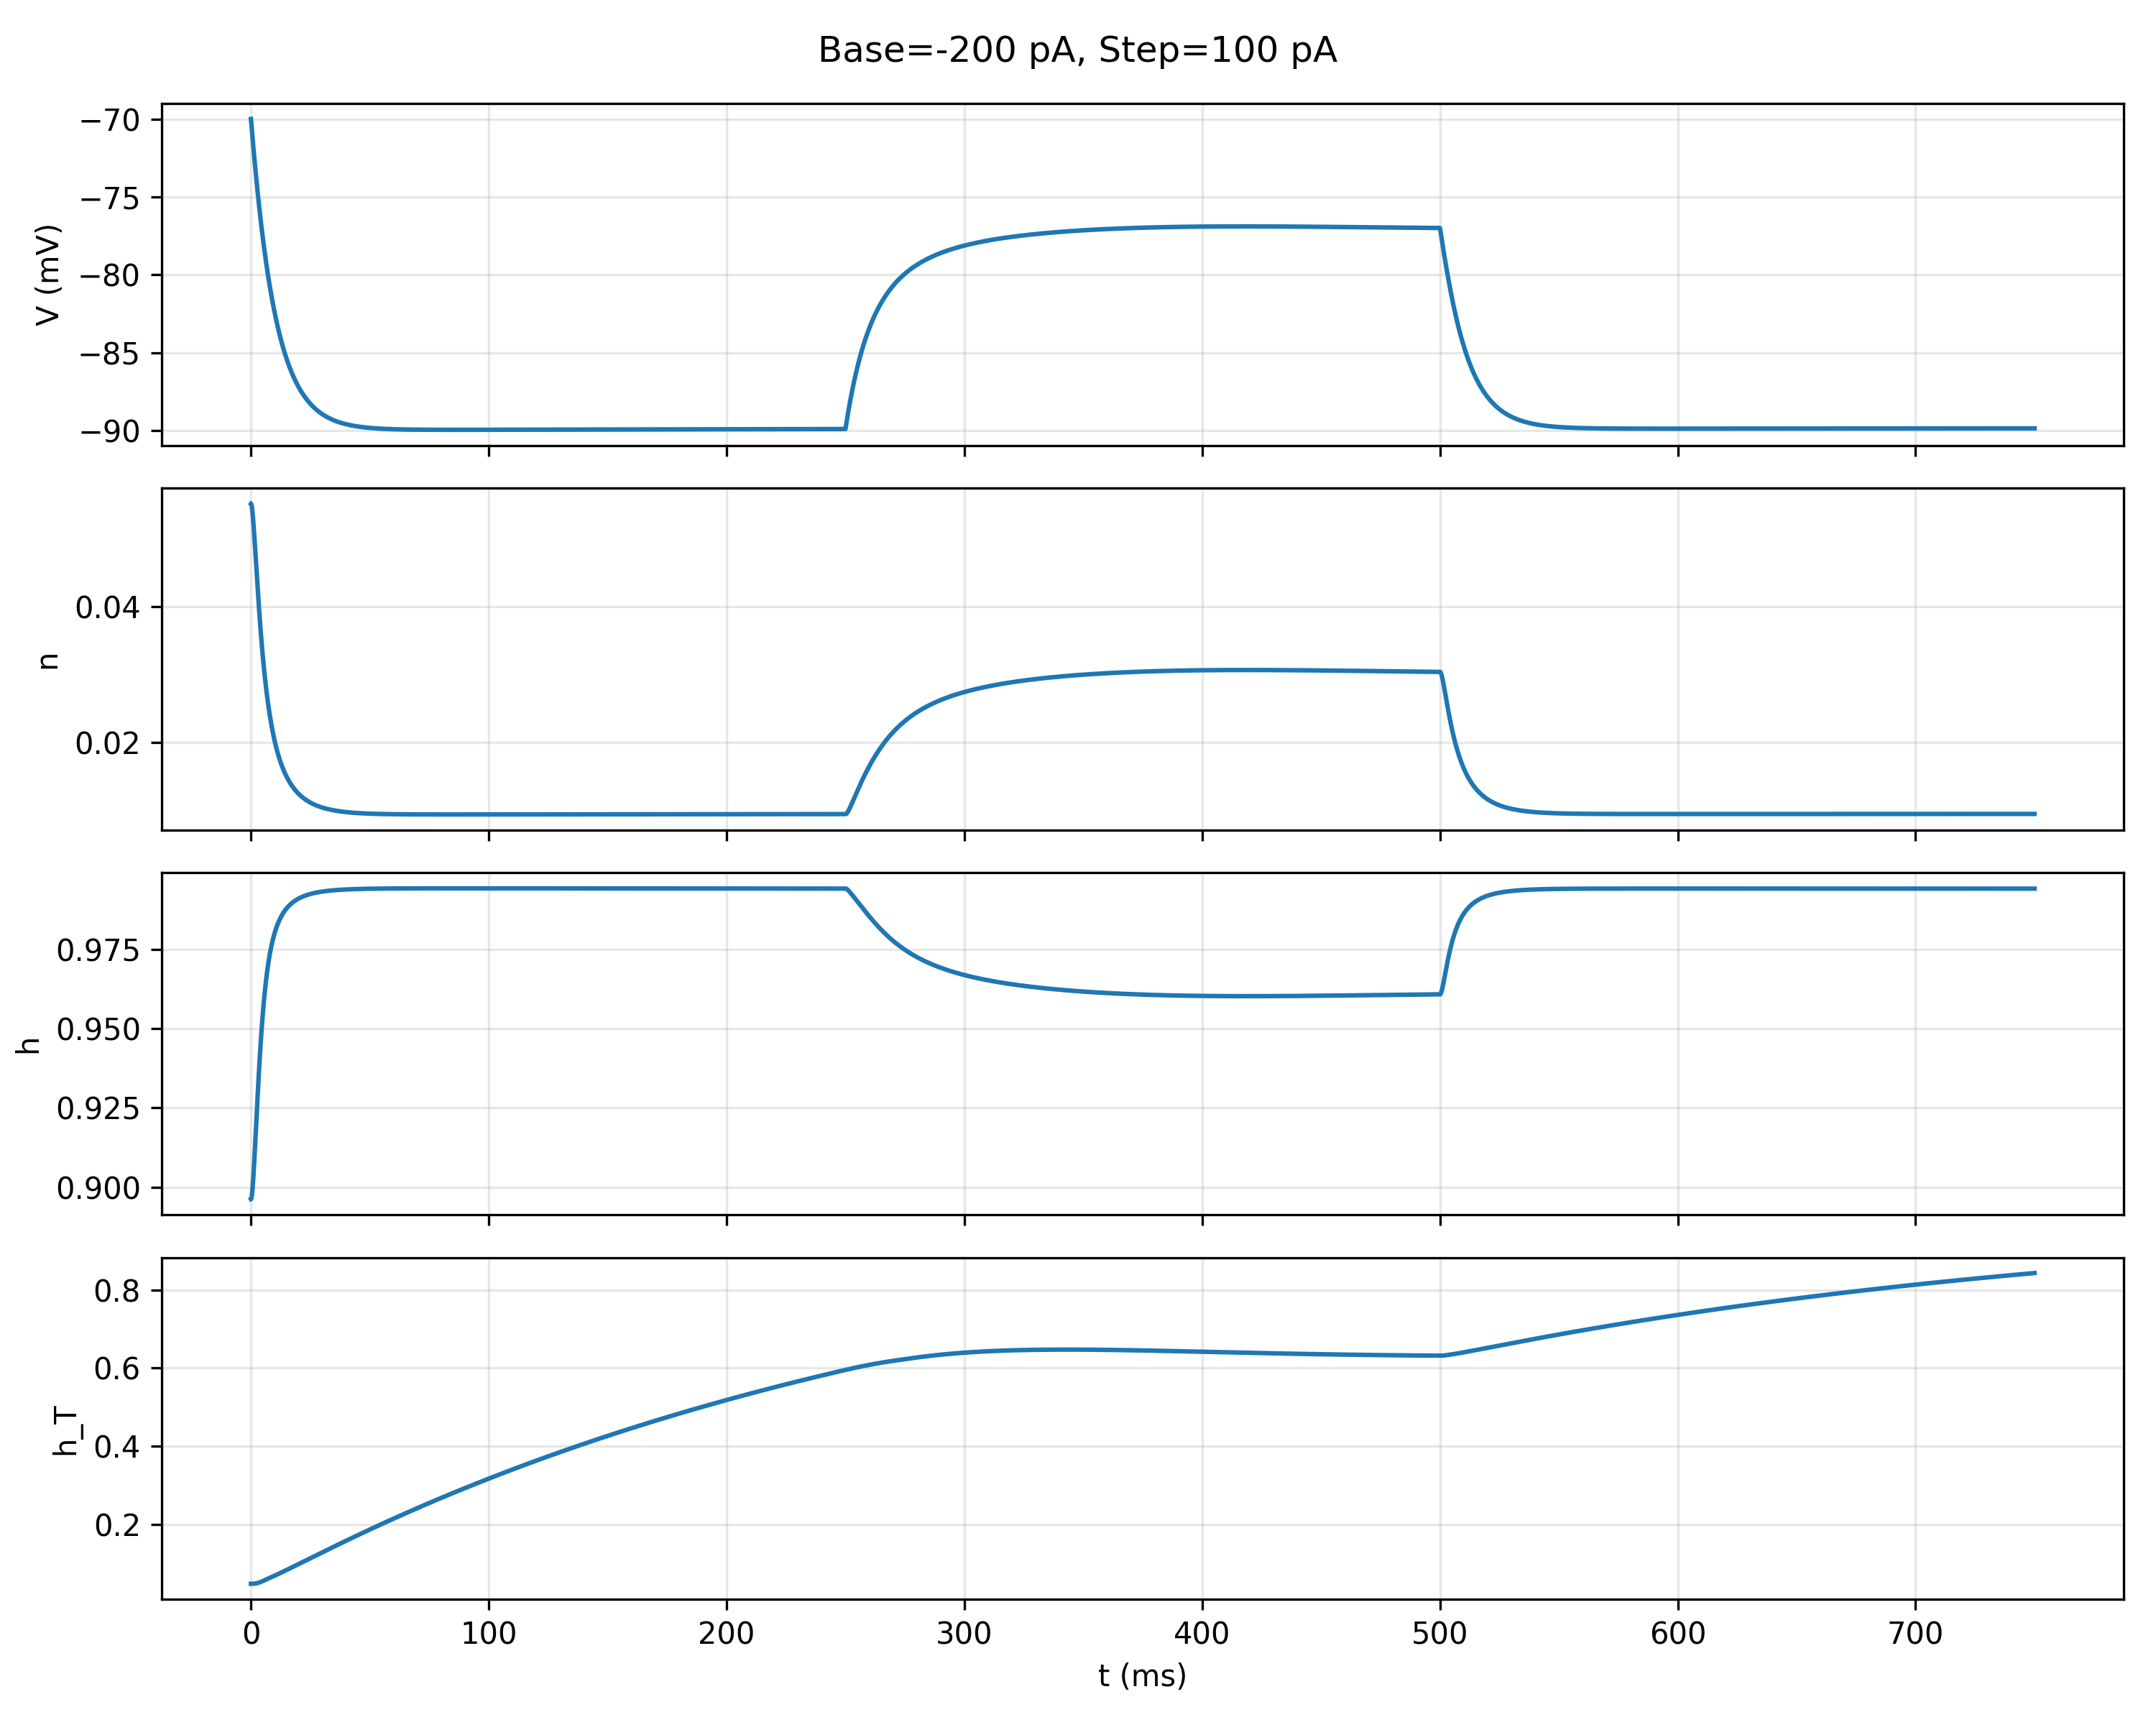
\includegraphics[width=11cm]{../figures/ex_2b_traces_base-200_step100.png}	
		\caption{Exemplo de comportamento com corrente base -200 pA e degrau 100 pA.}
	\end{figure}	
	\begin{figure}[H]
	\centering
	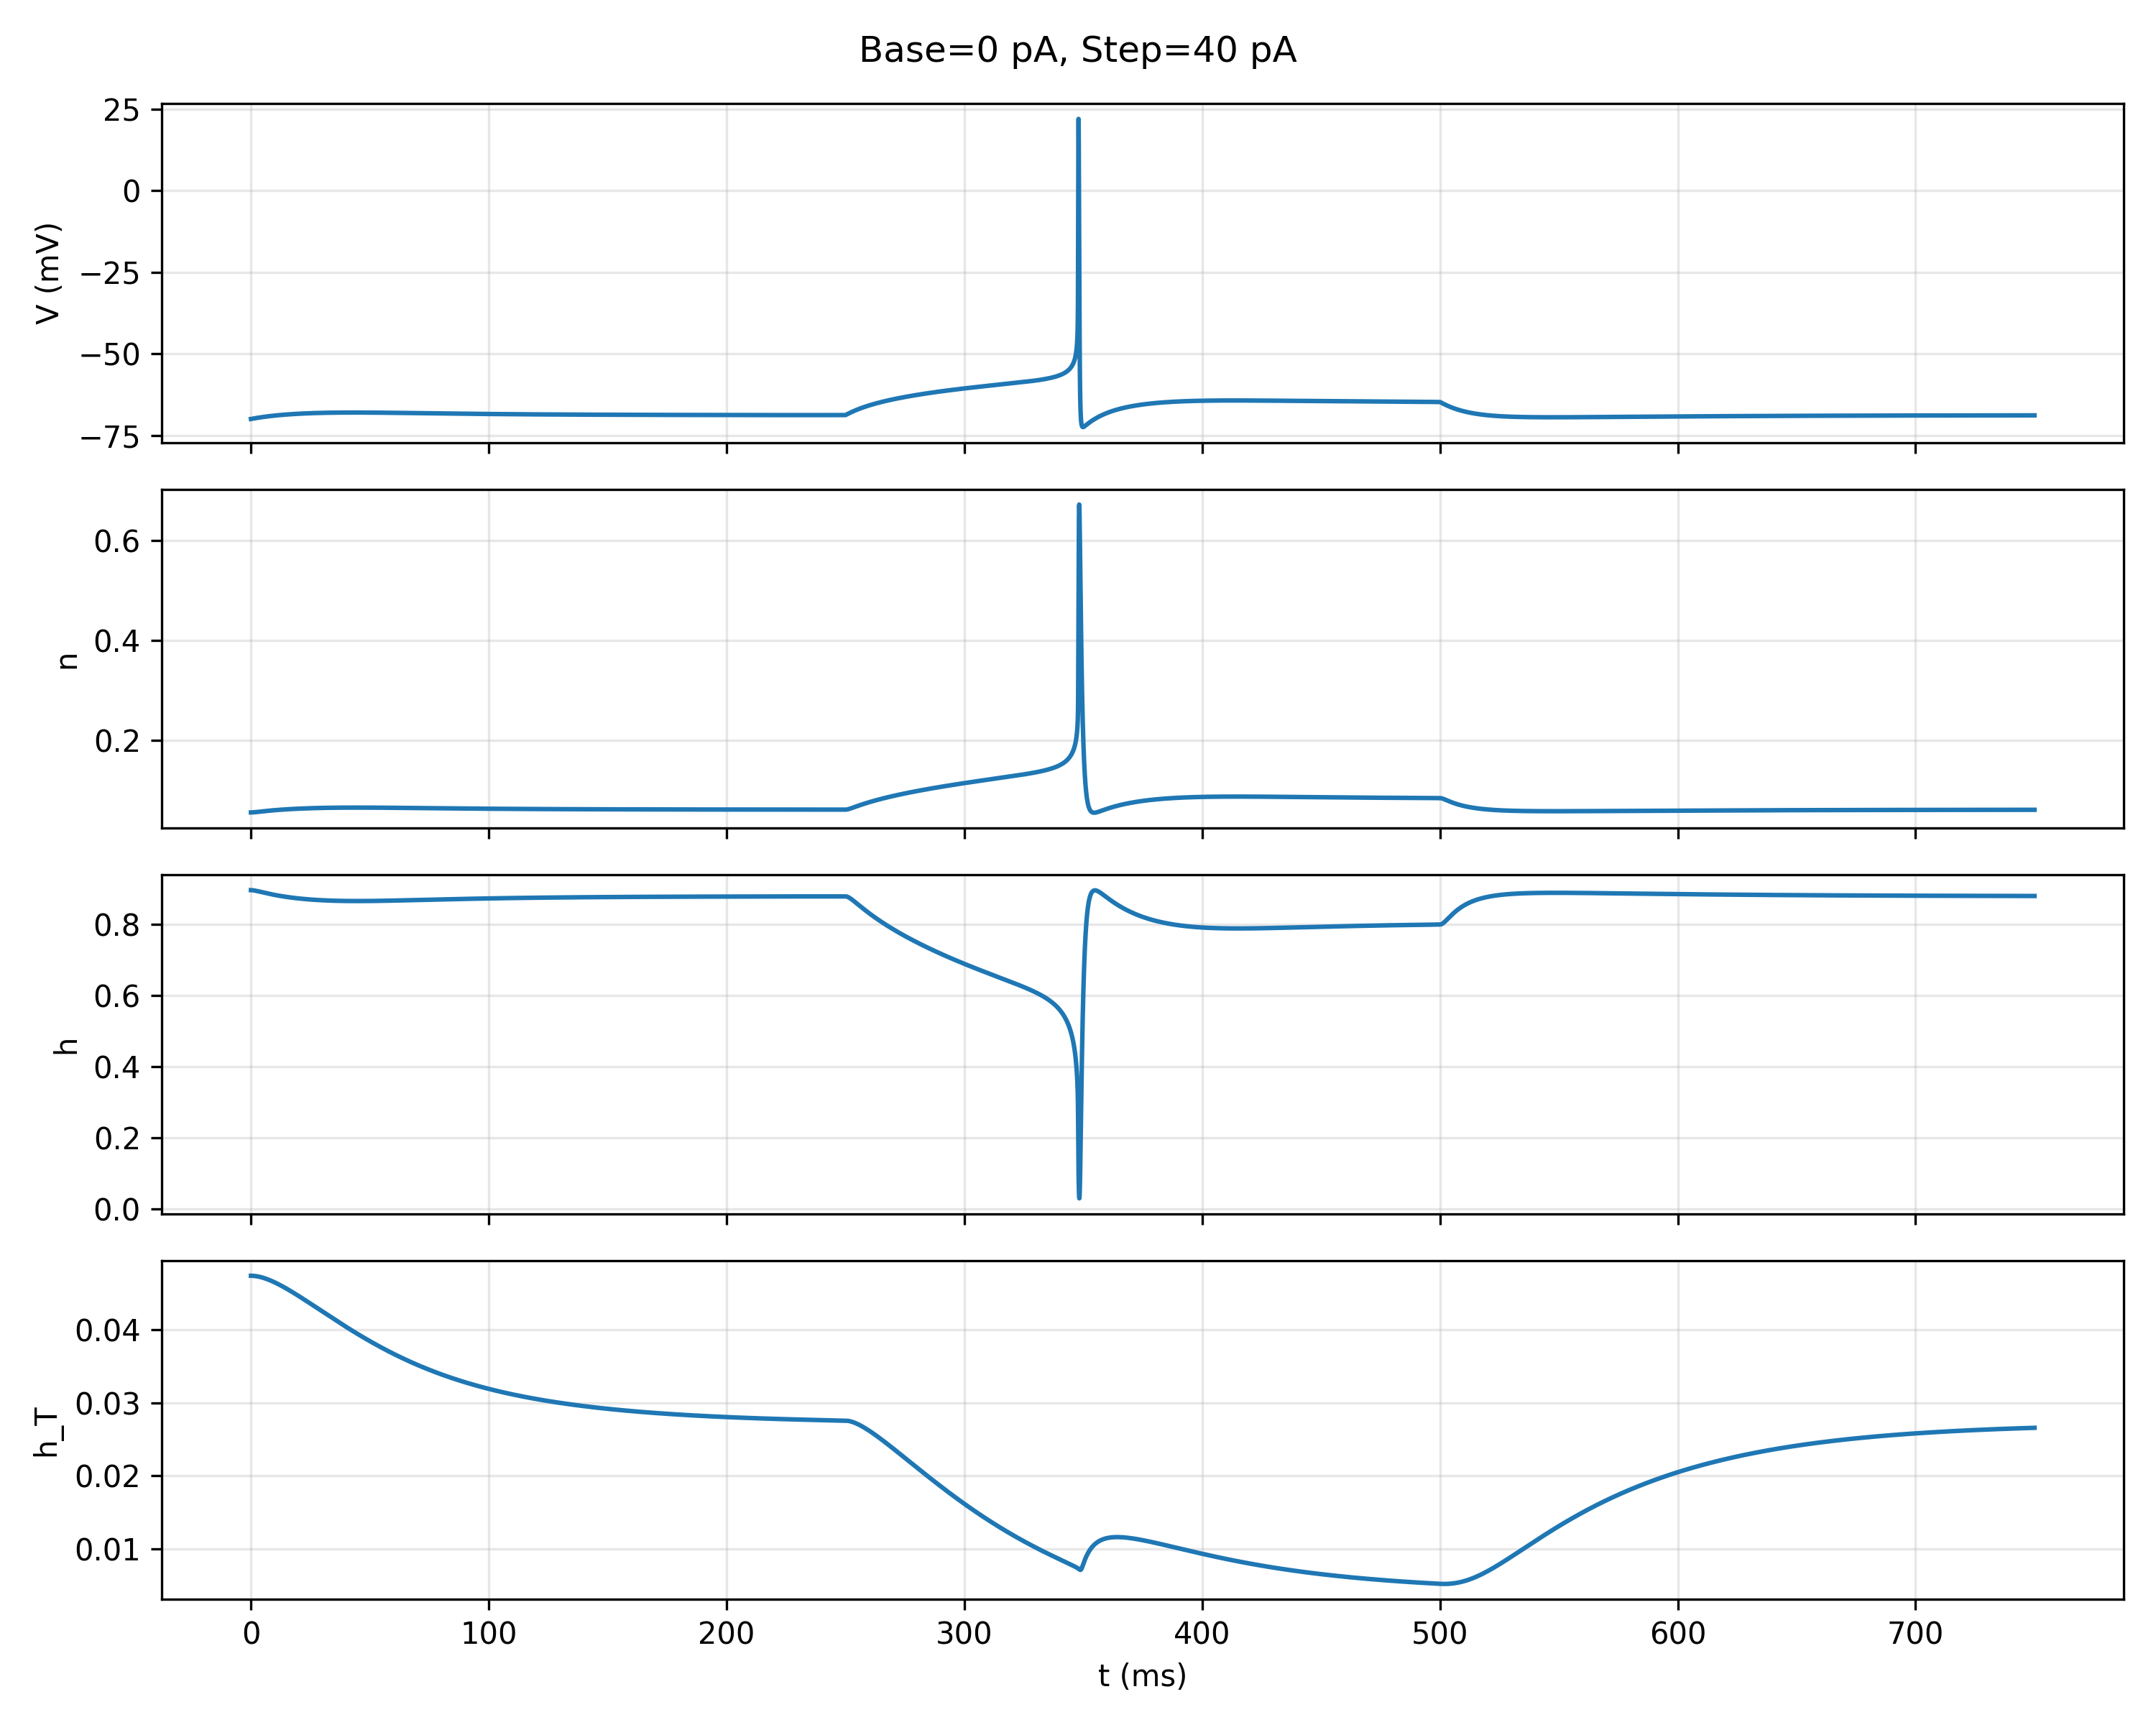
\includegraphics[width=11cm]{../figures/ex_2b_traces_base0_step40.png}	
	\caption{Exemplo de comportamento com corrente base 0 pA e degrau 40 pA.}
	\end{figure}	
	\begin{figure}[H]
	\centering
	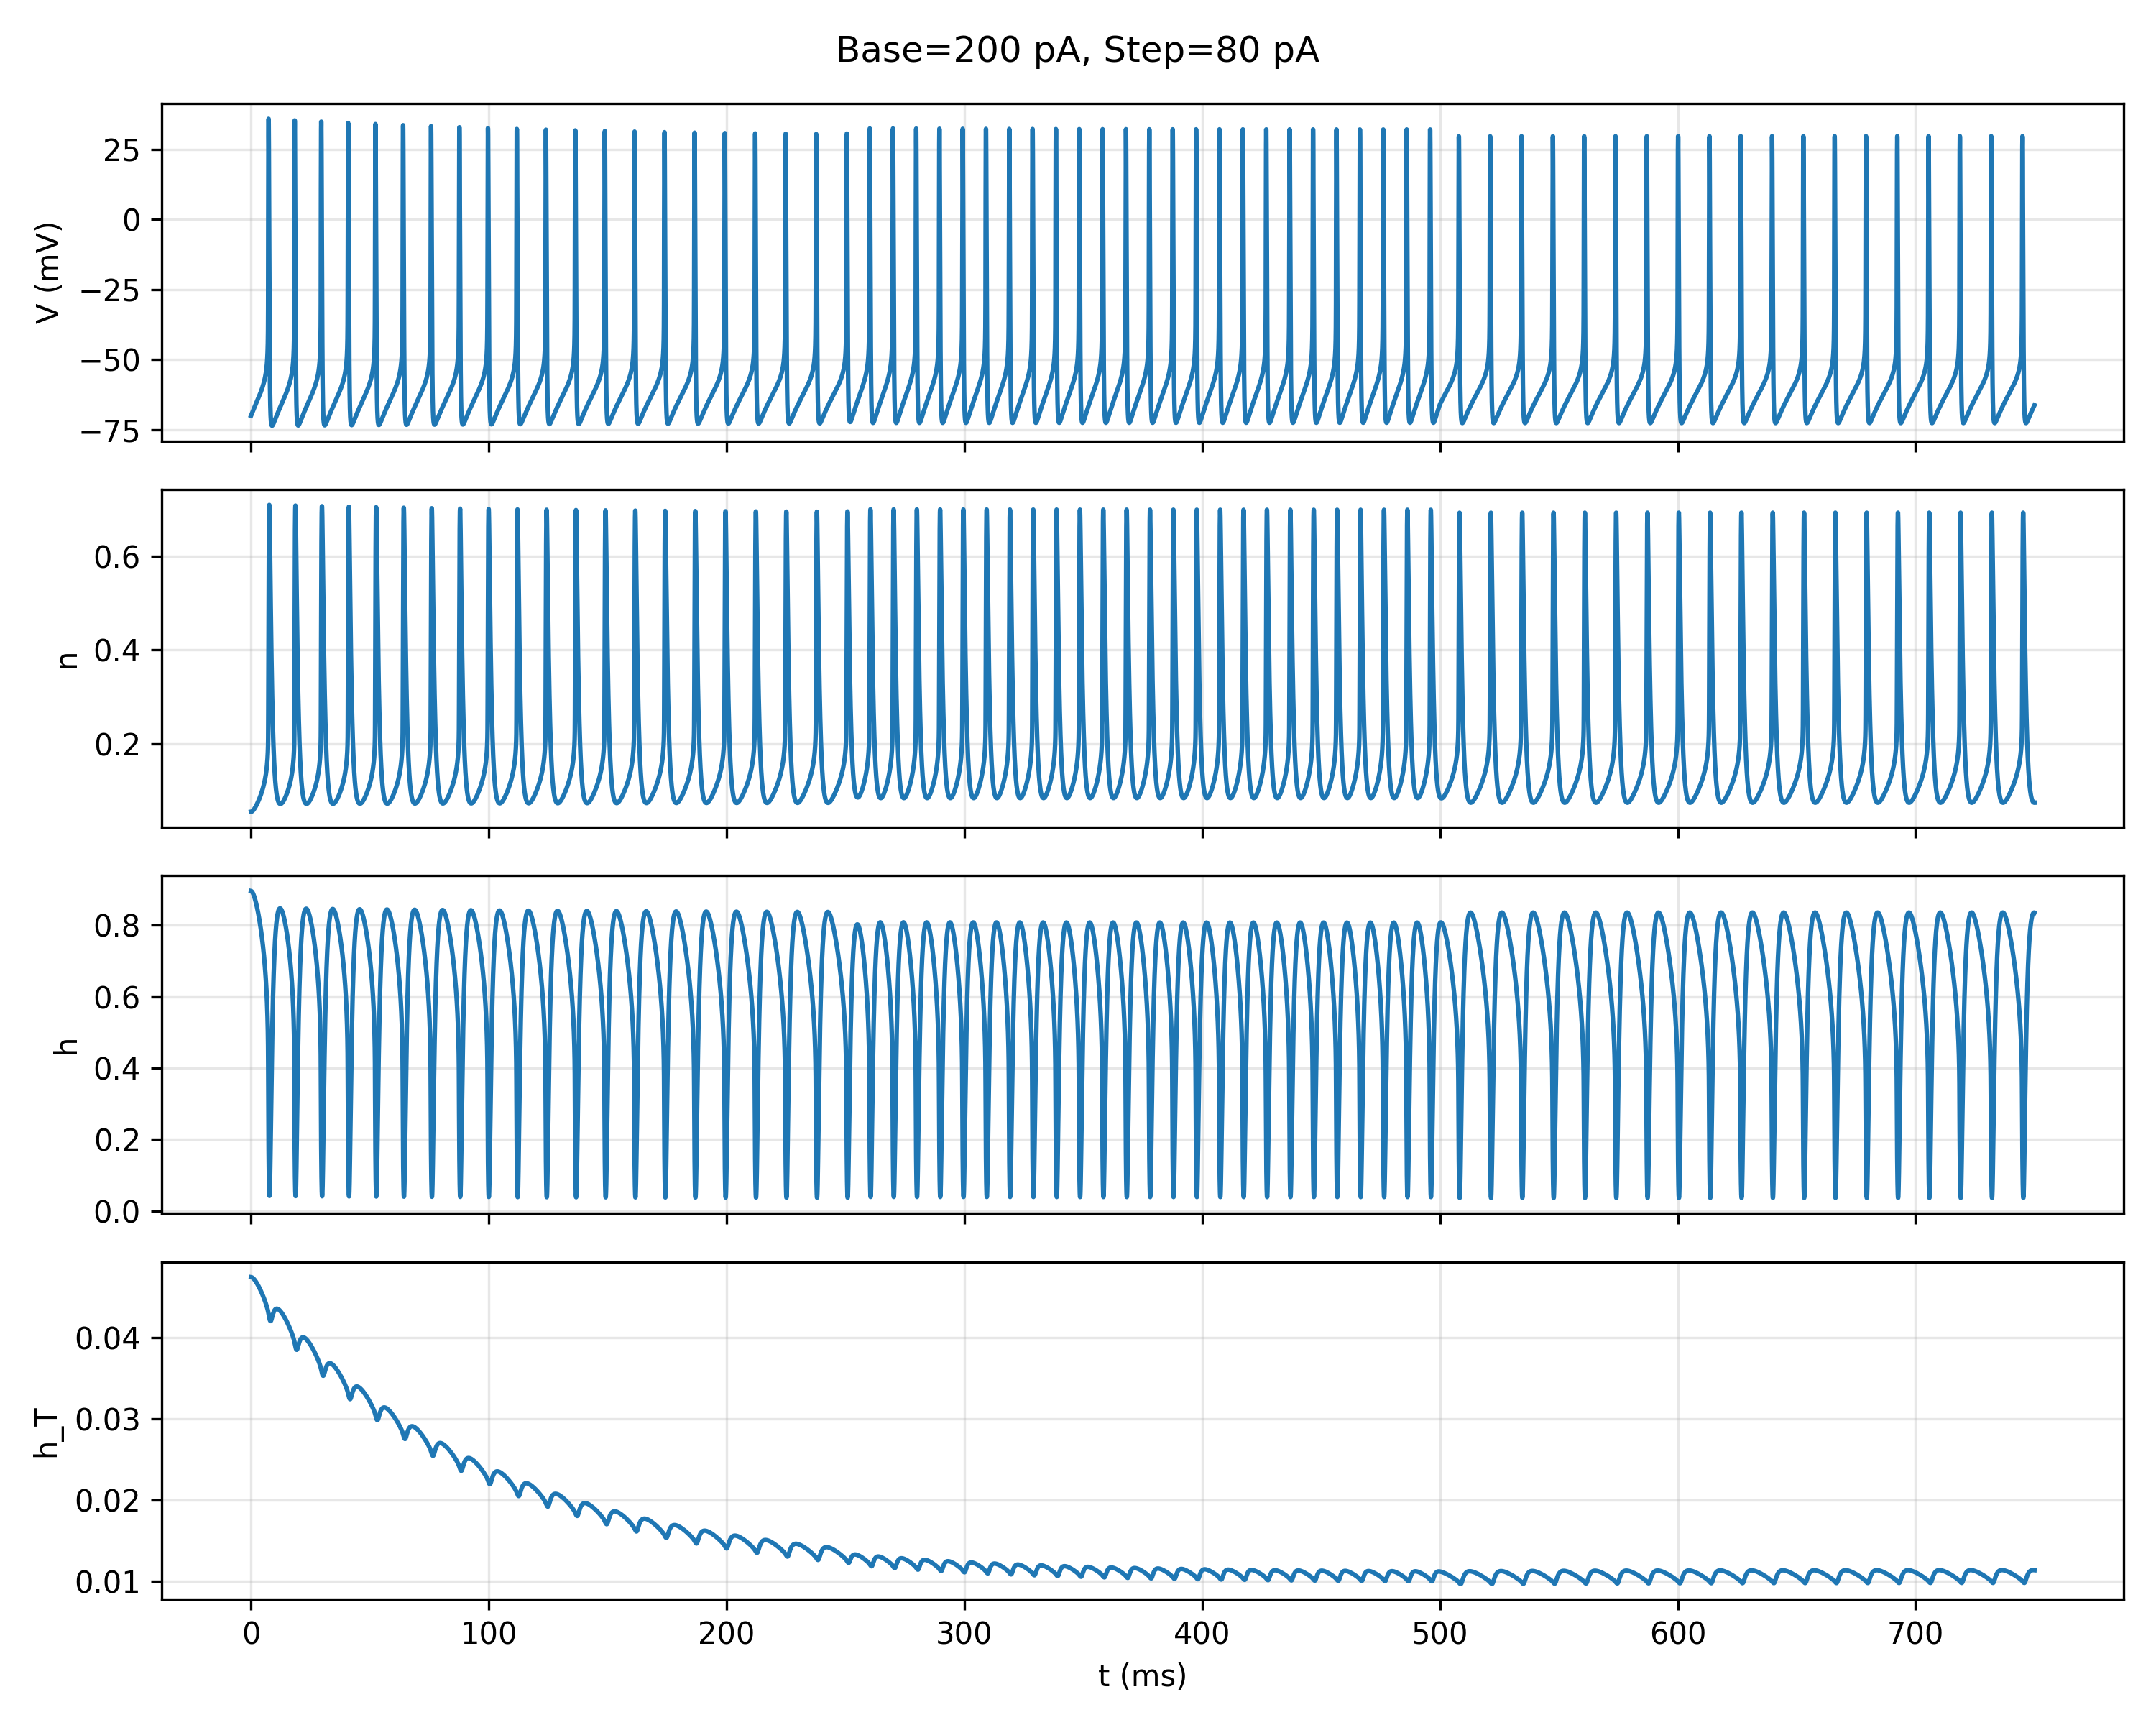
\includegraphics[width=11cm]{../figures/ex_2b_traces_base200_step80.png}	
	\caption{Exemplo de comportamento com corrente base 200 pA e degrau 80 pA.}
	\end{figure}
	
	
\end{document}